%%%  کلاس AUTthesis، نسخه آبان 1397
%%%   دانشگاه صنعتی امیرکبیر                 http://www.aut.ac.ir
%%%  تالار گفتگوی پارسی‌لاتک،       http://forum.parsilatex.com
%%%   آپدیت شده در آبان 295
%%%   پشتیبانی و راهنمایی          badali_farhad@yahoo.com
%%%
%%%   بازبینی و اصلاح شده در آبان ماه 1397
%%%  Tested via TeXstudio in TeXlive 2014-2018.
%%%

%-----------------------------------------------------------------------------------------------------
%        روش اجرا.: 2 بار F1 ، 2 بار  F11(به منظور تولید مراجع) ، دوبار Ctrl+Alt+I (به منظور تولید نمایه) و دو بار F1 -------> مشاهده Pdf
%%%%%%%%%%%%%%%%%%%%%%%%%%%%%%%%%%%%%%%%%%%%%%%%%%%%%%
%   TeXstudio as your IDE
%%  برای compile در TeXstudio تنها کافی است منوی Options->Configure TeXstudio را زده و در پنجره Configure TeXstudio در بخش Build گزینه Default Compiler را به XeLaTeX تغییر دهید. سند شما به راحتی compile خواهد شد.
%   F1 & F5 : Build & view
%   F6      : Compile
%   F7      : View
%   --------------
%%%%%%%%%%%%%%%%%%%%%%%%%%%%%%%%%%%%%%%%%%%%%%%%%%%%%%
%        اگر قصد نوشتن رساله دکتری را دارید، در خط زیر به جای msc،
%      کلمه phd را قرار دهید. کلیه تنظیمات لازم، به طور خودکار، اعمال می‌شود.
%%% !TEX TS-program = XeLaTeX
\documentclass[oneside,bsc,12pt]{AUTthesis}
%       فایل commands.tex را حتماً به دقت مطالعه کنید؛ چون دستورات مربوط به فراخوانی بسته زی‌پرشین 
%       و دیگر بسته‌ها و ... در این فایل قرار دارد و بهتر است که با نحوه استفاده از آنها آشنا شوید. توجه شود برای نسخه نهایی پایان‌نامه حتماً hyperref را 
%        غیرفعال کنید.


% در این فایل، دستورها و تنظیمات مورد نیاز، آورده شده است.
%-------------------------------------------------------------------------------------------------------------------
% در ورژن جدید زی‌پرشین برای تایپ متن‌های ریاضی، این سه بسته، حتماً باید فراخوانی شود.
\usepackage{amsthm,amssymb,amsmath,amsfonts}
% بسته‌ای برای تنطیم حاشیه‌های بالا، پایین، چپ و راست صفحه
\usepackage[top=30mm, bottom=30mm, left=25mm, right=30mm]{geometry}
% بسته‌‌ای برای ظاهر شدن شکل‌ها و تصاویر متن
\usepackage{graphicx}
\usepackage{color}
\usepackage{multirow}
%بسته‌ای برای تنظیم فاصله عمودی خط‌های متن
\usepackage{setspace}
\usepackage{titletoc}
\usepackage[round]{natbib}

\usepackage[utf8]{inputenc}
\usepackage{fourier} 
\usepackage{array}
\usepackage{makecell}

\renewcommand\theadalign{bc}
\renewcommand\theadfont{\bfseries}
\renewcommand\theadgape{\Gape[4pt]}
\renewcommand\cellgape{\Gape[4pt]}


\usepackage{subcaption}
\usepackage{tocloft}
%با فعال کردن بسته زیر فوت‌نوت‌ها در هر صفحه ریست می‌شوند. حالت پیش‌فرض آن ریست شدن در هر فصل می‌باشد.
%\usepackage[perpage]{footmisc}
\usepackage{enumitem}
%\usepackage{titlesec}
% بسته‌ و دستوراتی برای ایجاد لینک‌های رنگی با امکان جهش
\usepackage[pagebackref=false,colorlinks,linkcolor=blue,citecolor=red]{hyperref}
\usepackage[nameinlink]{cleveref}%capitalize,,noabbrev
 \AtBeginDocument{%
    \crefname{equation}{برابری}{equations}%
    \crefname{chapter}{فصل}{chapters}%
    \crefname{section}{بخش}{sections}%
    \crefname{appendix}{پیوست}{appendices}%
    \crefname{enumi}{مورد}{items}%
    \crefname{footnote}{زیرنویس}{footnotes}%
    \crefname{figure}{شکل}{figures}%
    \crefname{table}{جدول}{tables}%
    \crefname{theorem}{قضیه}{theorems}%
    \crefname{lemma}{لم}{lemmas}%
    \crefname{corollary}{نتیجه}{corollaries}%
    \crefname{proposition}{گزاره}{propositions}%
    \crefname{definition}{تعریف}{definitions}%
    \crefname{result}{نتیجه}{results}%
    \crefname{example}{مثال}{examples}%
    \crefname{remark}{نکته}{remarks}%
    \crefname{note}{یادداشت}{notes}%
}
% چنانچه قصد پرینت گرفتن نوشته خود را دارید، خط بالا را غیرفعال و  از دستور زیر استفاده کنید چون در صورت استفاده از دستور زیر‌‌، 
% لینک‌ها به رنگ سیاه ظاهر خواهند شد که برای پرینت گرفتن، مناسب‌تر است
%\usepackage[pagebackref=false]{hyperref}
% بسته‌ لازم برای تنظیم سربرگ‌ها
\usepackage{fancyhdr}
% بسته‌ای برای ظاهر شدن «مراجع»  در فهرست مطالب
\usepackage[nottoc]{tocbibind}
% دستورات مربوط به ایجاد نمایه
\usepackage{makeidx,multicol}
\setlength{\columnsep}{1.5cm}

%%%%%%%%%%%%%%%%%%%%%%%%%%
\usepackage{verbatim}
\makeindex
\usepackage{sectsty}
% فراخوانی بسته زی‌پرشین و تعریف قلم فارسی و انگلیسی
\usepackage{xepersian}%[extrafootnotefeatures]
\SepMark{-}
%حتماً از تک لایو 2014 استفاده کنید.
\settextfont[Scale=1.2]{B Nazanin}
%\setlatintextfont{Times New Roman}
\renewcommand{\labelitemi}{$\bullet$}
%%%%%%%%%%%%%%%%%%%%%%%%%%
% چنانچه می‌خواهید اعداد در فرمول‌ها، انگلیسی باشد، خط زیر را غیرفعال کنید.
%در غیر اینصورت حتماً فونت PGaramond را نصب کنید.
%\setdigitfont[Scale=1.1]{PGaramond}%%Yas
%%%%%%%%%%%%%%%%%%%%%%%%%%
% تعریف قلم‌های فارسی اضافی برای استفاده در بعضی از قسمت‌های متن
\defpersianfont\nastaliq[Scale=2]{IranNastaliq}
\defpersianfont\chapternumber[Scale=3]{B Nazanin}
%\chapterfont{\centering}%
%%%%%%%%%%%%%%%%%%%%%%%%%%
% دستوری برای تغییر نام کلمه «اثبات» به «برهان»
\renewcommand\proofname{\textbf{برهان}}

% دستوری برای تغییر نام کلمه «کتاب‌نامه» به «منابع و مراجع«
\renewcommand{\bibname}{منابع و مراجع}


% Headings for every page of ToC, LoF and Lot
\setlength{\cftbeforetoctitleskip}{-1.2em}
\setlength{\cftbeforelottitleskip}{-1.2em}
\setlength{\cftbeforeloftitleskip}{-1.2em}
\setlength{\cftaftertoctitleskip}{-1em}
\setlength{\cftafterlottitleskip}{-1em}
\setlength{\cftafterloftitleskip}{-1em}
%%\makeatletter
%%%%\renewcommand{\l@chapter}{\@dottedtocline{1}{1em\bfseries}{1em}}
%%%%\renewcommand{\l@section}{\@dottedtocline{2}{2em}{2em}}
%%%%\renewcommand{\l@subsection}{\@dottedtocline{3}{3em}{3em}}
%%%%\renewcommand{\l@subsubsection}{\@dottedtocline{4}{4em}{4em}}
%%%%\makeatother


\newcommand\tocheading{\par عنوان\hfill صفحه \par}
\newcommand\lofheading{\hspace*{.5cm}\figurename\hfill صفحه \par}
\newcommand\lotheading{\hspace*{.5cm}\tablename\hfill صفحه \par}

\renewcommand{\cftchapleader}{\cftdotfill{\cftdotsep}}
\renewcommand{\cfttoctitlefont}{\hspace*{\fill}\LARGE\bfseries}%\Large
\renewcommand{\cftaftertoctitle}{\hspace*{\fill}}
\renewcommand{\cftlottitlefont}{\hspace*{\fill}\LARGE\bfseries}%\Large
\renewcommand{\cftafterlottitle}{\hspace*{\fill}}
\renewcommand{\cftloftitlefont}{\hspace*{\fill}\LARGE\bfseries}
\renewcommand{\cftafterloftitle}{\hspace*{\fill}}

%%%%%%%%%%%%%%%%%%%%%%%%%%
% تعریف و نحوه ظاهر شدن عنوان قضیه‌ها، تعریف‌ها، مثال‌ها و ...
%برای شماره گذاری سه تایی قضیه ها
\theoremstyle{definition}
\newtheorem{definition}{تعریف}[section]
\newtheorem{remark}[definition]{نکته}
\newtheorem{note}[definition]{یادداشت}
\newtheorem{example}[definition]{نمونه}
\newtheorem{question}[definition]{سوال}
\newtheorem{remember}[definition]{یاداوری}
%\theoremstyle{theorem}
\newtheorem{theorem}[definition]{قضیه}
\newtheorem{lemma}[definition]{لم}
\newtheorem{proposition}[definition]{گزاره}
\newtheorem{corollary}[definition]{نتیجه}
%%%%%%%%%%%%%%%%%%%%%%%%
%%%%%%%%%%%%%%%%%%%
%%% برای شماره گذاری چهارتایی قضیه ها و ...
%%\newtheorem{definition1}[subsubsection]{تعریف}
%%\newtheorem{theorem1}[subsubsection]{قضیه}
%%\newtheorem{lemma1}[subsubsection]{لم}
%%\newtheorem{proposition1}[subsubsection]{گزاره}
%%\newtheorem{corollary1}[subsubsection]{نتیجه}
%%\newtheorem{remark1}[subsubsection]{نکته}
%%\newtheorem{example1}[subsubsection]{مثال}
%%\newtheorem{question1}[subsubsection]{سوال}

%%%%%%%%%%%%%%%%%%%%%%%%%%%%

% دستورهایی برای سفارشی کردن صفحات اول فصل‌ها
\makeatletter
\newcommand\mycustomraggedright{%
 \if@RTL\raggedleft%
 \else\raggedright%
 \fi}
\def\@makechapterhead#1{%
\thispagestyle{style1}
\vspace*{20\p@}%
{\parindent \z@ \mycustomraggedright
\ifnum \c@secnumdepth >\m@ne
\if@mainmatter

\bfseries{\Huge \@chapapp}\small\space {\chapternumber\thechapter}
\par\nobreak
\vskip 0\p@
\fi
\fi
\interlinepenalty\@M 
\Huge \bfseries #1\par\nobreak
\vskip 120\p@

}

%\thispagestyle{empty}
\newpage}
\bidi@patchcmd{\@makechapterhead}{\thechapter}{\tartibi{chapter}}{}{}
\bidi@patchcmd{\chaptermark}{\thechapter}{\tartibi{chapter}}{}{}
\makeatother

\pagestyle{fancy}
\renewcommand{\chaptermark}[1]{\markboth{\chaptername~\tartibi{chapter}: #1}{}}

\fancypagestyle{style1}{
\fancyhf{} 
\fancyfoot[c]{\thepage}
\fancyhead[R]{\leftmark}%
\renewcommand{\headrulewidth}{1.2pt}
}


\fancypagestyle{style2}{
\fancyhf{}
\fancyhead[R]{چکیده}
\fancyfoot[C]{\thepage{}}
\renewcommand{\headrulewidth}{1.2pt}
}

\fancypagestyle{style3}{%
  \fancyhf{}%
  \fancyhead[R]{فهرست نمادها}
  \fancyfoot[C]{\thepage}%
  \renewcommand{\headrulewidth}{1.2pt}%
}

\fancypagestyle{style4}{%
  \fancyhf{}%
  \fancyhead[R]{فهرست جداول}
  \fancyfoot[C]{\thepage}%
  \renewcommand{\headrulewidth}{1.2pt}%
}

\fancypagestyle{style5}{%
  \fancyhf{}%
  \fancyhead[R]{فهرست اشکال}
  \fancyfoot[C]{\thepage}%
  \renewcommand{\headrulewidth}{1.2pt}%
}

\fancypagestyle{style6}{%
  \fancyhf{}%
  \fancyhead[R]{فهرست مطالب}
  \fancyfoot[C]{\thepage}%
  \renewcommand{\headrulewidth}{1.2pt}%
}

\fancypagestyle{style7}{%
  \fancyhf{}%
  \fancyhead[R]{نمایه}
  \fancyfoot[C]{\thepage}%
  \renewcommand{\headrulewidth}{1.2pt}%
}

\fancypagestyle{style8}{%
  \fancyhf{}%
  \fancyhead[R]{منابع و مراجع}
  \fancyfoot[C]{\thepage}%
  \renewcommand{\headrulewidth}{1.2pt}%
}
\fancypagestyle{style9}{%
  \fancyhf{}%
  \fancyhead[R]{واژه‌نامه‌ی فارسی به انگلیسی}
  \fancyfoot[C]{\thepage}%
  \renewcommand{\headrulewidth}{1.2pt}%
}
%


%دستور حذف نام لیست تصاویر و لیست جداول از فهرست مطالب
\newcommand*{\BeginNoToc}{%
  \addtocontents{toc}{%
    \edef\protect\SavedTocDepth{\protect\the\protect\value{tocdepth}}%
  }%
  \addtocontents{toc}{%
    \protect\setcounter{tocdepth}{-10}%
  }%
}
\newcommand*{\EndNoToc}{%
  \addtocontents{toc}{%
    \protect\setcounter{tocdepth}{\protect\SavedTocDepth}%
  }%
}
\newcounter{savepage}
\renewcommand{\listfigurename}{فهرست اشکال}
\renewcommand{\listtablename}{فهرست جداول}
%\renewcommand\cftsecleader{\cftdotfill{\cftdotsep}}
%%%%%%%%%%%%%%%%%%%%%%%%%%%%%
%%%%%%%%%%%%%%%%%%%%%%%%%%%%


\begin{document}
\baselineskip=.75cm
\linespread{1.75}
%% -!TEX root = AUTthesis.tex
% در این فایل، عنوان پایان‌نامه، مشخصات خود، متن تقدیمی‌، ستایش، سپاس‌گزاری و چکیده پایان‌نامه را به فارسی، وارد کنید.
% توجه داشته باشید که جدول حاوی مشخصات پروژه/پایان‌نامه/رساله و همچنین، مشخصات داخل آن، به طور خودکار، درج می‌شود.
%%%%%%%%%%%%%%%%%%%%%%%%%%%%%%%%%%%%
% دانشکده، آموزشکده و یا پژوهشکده  خود را وارد کنید
\faculty{دانشکده مهندسی کامپیوتر}
% گرایش و گروه آموزشی خود را وارد کنید
\department{گرایش هوش مصنوعی}
% عنوان پایان‌نامه را وارد کنید
\fatitle{پیش‌بینی نوسان قیمت در بازار رمزارزها با استفاده از یادگیري عمیق
	\\[.75 cm]
	پایان‌نامه}
% نام استاد(ان) راهنما را وارد کنید
\firstsupervisor{دکتر مریم امیرمزلقانی}
%\secondsupervisor{استاد راهنمای دوم}
% نام استاد(دان) مشاور را وارد کنید. چنانچه استاد مشاور ندارید، دستور پایین را غیرفعال کنید.
%\firstadvisor{نام کامل استاد مشاور}
%\secondadvisor{استاد مشاور دوم}
% نام نویسنده را وارد کنید
\name{سید علیرضا }
% نام خانوادگی نویسنده را وارد کنید
\surname{بختیاری}
%%%%%%%%%%%%%%%%%%%%%%%%%%%%%%%%%%
\thesisdate{تیر ۱۴۰۰}

% چکیده پایان‌نامه را وارد کنید
\fa-abstract{
	هدف از انجام این پروژه پیش‌بینی نوسان قیمت در بازار رمزارزها با استفاده از اطلاعات دفتر ثبت سفارشات و شبکه‌هاي عمیق بازگشتی است. پیشبینی نوسان در بازارهاي مالی به طور کلی از اهمیت زیادي برخوردار است. به صورت سنتی تنها از اطلاعات قیمت براي محاسبه‌ي نوسان در مدلهاي آماري استفاده شده‌است. از طرفی استفاده از اطلاعات موجود در دفتر ثبت سفارشات که شامل تمامی سفارشات موجود و در جریان یک بازار است می‌تواند دقت این مدل‌ها افزایش دهد. اما به دلیل حجم زیاد این داده ساختارها،‌ در گذشته کمتر از آن‌ها در جهت پیش‌بینی نوسان استفاده شده است.\\
	در این پروژه با واکشی و پیش‌پردازش اطلاعات دفتر ثبت سفارشات و سپس با استفاده از مدلهاي یادگیري عمیق بازگشتی، سعی در مدل کردن نوسان در بازارهاي رمزارزها را داریم. نتایج به دست آمده نشان‌دهنده‌ی برتری مدل‌های یادگیری عمیق بازگشتی در مقایسه با دیگر معماری‌های شبکه‌های عصبی در پیش‌بینی نوسان هستند.
}


% کلمات کلیدی پایان‌نامه را وارد کنید
\keywords{پیش‌بینی سری‌‌های‌ زمانی، نوسان قیمت،‌ شبکه‌های عصبی، یادگیری عمیق،‌شبکه‌های عمیق بازگشتی، دفتر ثبت سفارشات}



\AUTtitle
%%%%%%%%%%%%%%%%%%%%%%%%%%%%%%%%%%
\vspace*{7cm}
\thispagestyle{empty}
\begin{center}
	\nastaliq{\huge{به نام خدا}}
\end{center}
% تاییدیه دفاع
\newpage
\thispagestyle{empty}
%\fontsize{18pt}{19pt}\selectfont

\section*{صفحه فرم ارزیابی و تصویب پایان نامه- فرم تأیید اعضاء كميته دفاع}

\fontsize{12pt}{14pt}\selectfont
%\renewcommand{\baselinestretch}{1.5}
\vspace*{1cm}
   در این صفحه فرم دفاع یا تایید و تصویب پایان نامه موسوم به فرم کمیته دفاع- موجود در پرونده آموزشی- را قرار دهید.
\vspace*{1cm}


\subsection*{نکات مهم:}
 
\begin{itemize}
\item
	نگارش پایان نامه/رساله باید به
	{\color{red}
		زبان فارسی
	}
	و بر اساس آخرین نسخه دستورالعمل و راهنمای تدوین پایان نامه های دانشگاه صنعتی امیرکبیر باشد.(دستورالعمل و راهنمای حاضر)
\item رنگ جلد پایان نامه/رساله چاپي كارشناسي، كارشناسي ارشد و دكترا  بايد به ترتيب مشكي، طوسي و سفيد رنگ باشد.  
\item چاپ و صحافی پایان نامه/رساله بصورت
{\color{red}
	پشت و رو(دورو)
}
بلامانع است و انجام آن توصيه مي شود. 
\end{itemize}
%%%%%%%%%%%%%%%%%%%%%%%%%%%%%%%%%%%%%%%%%%%%%%%%%%%%%%%%%%%%%%%%%%%%%%%%%%%%%%%%%%%%%%%%%%%%%%%%%%
%%%%%%%%%%%%%%%%%%%%%%%%%%%%%%%%%%%%%%%%%%%%%%%%%%%%%%%%%%%%%%%%%%%%%%%%%%%%%%%%%%%%%%%%%%%%%%%%%%
\newpage
\thispagestyle{empty}
\begin{picture}(50,50)
  \put(17,0){
\includegraphics[scale=1.1]{fa-logo}}
  \put(4.5,-13){\footnotesize{دانشگاه صنعتی امیرکبیر}}
  \put(10.5,-27){\footnotesize{(پلی‌تکنیک تهران)}}
  \put(170,30){\bf{به نام خدا}}
  \put(140,-5){\Large\bf{تعهدنامه اصالت اثر}}
  \put(310,0){تاریخ: \datethesis}
\end{picture}

\vspace*{2.5cm}

اينجانب {\bf{\fname\lname}} متعهد می‌شوم که مطالب مندرج در این پایان‌نامه حاصل کار پژوهشی اینجانب تحت نظارت و راهنمایی اساتید دانشگاه صنعتی امیرکبیر بوده و به دستاوردهای دیگران که در این پژوهش از آن‌ها استفاده شده است مطابق مقررات و روال متعارف ارجاع و در فهرست منابع و مآخذ ذکر گردیده است. این پایان‌نامه قبلاً برای احراز هیچ مدرک هم‌سطح یا بالاتر ارائه نگردیده است.

در صورت اثبات تخلف در هر زمان، مدرک تحصیلی صادر شده توسط دانشگاه از درجه اعتبار ساقط بوده و دانشگاه حق پیگیری قانونی خواهد داشت.


کلیه نتایج و حقوق حاصل از این پایان‌نامه متعلق به دانشگاه صنعتی امیرکبیر می‌باشد. هرگونه استفاده از نتایج علمی و عملی، واگذاری اطلاعات به دیگران یا چاپ و تکثیر، نسخه‌برداری، ترجمه و اقتباس از این پایان نامه بدون موافقت کتبی دانشگاه صنعتی امیرکبیر ممنوع است. 
نقل مطالب با ذکر مآخذ بلامانع است.\\
\vspace{2.5cm}


{\centerline {\bf{\fname\lname}}}
\vspace*{.2cm}
{\centerline{امضا}}
%%%%%%%%%%%%%%%%%%%%%%%%%%%%%%%%%
% چنانچه مایل به چاپ صفحات «تقدیم»، «نیایش» و «سپاس‌گزاری» در خروجی نیستید، خط‌های زیر را با گذاشتن ٪  در ابتدای آنها غیرفعال کنید.
% پایان‌نامه خود را تقدیم کنید
% نیایش خود را در فایل زیر بنویسید.
%\begin{acknowledgementpage}

\vspace{1.5cm}

{\nastaliq
{
 نويسنده پايان‌نامه، درصورت تمايل ميتواند برای سپاسگزاری پايان‌نامه خود را به يا اشخاص و يا ارگان خاصی تقدیم نماید.
}}\end{acknowledgementpage}
\newpage
% سپاسگزاری را در فایل زیر بنویسید.
%%%%%%%%%%%%%%%%%%%%%%%%%%%%%%%%%%%%
\newpage\thispagestyle{empty}
% سپاس‌گزاری
{\nastaliq
سپاس‌گزاری
}
\\[2cm]
اکنون که مراحل پژوهش، تدوین و نگارش پایان نامه به پایان رسیده است، از مادر و پدر عزیزتر از جانم متشکرم که درطول زندگی و دوران تحصیل همراه و مشوقم بوده‌اند و با ایثار و از خودگذشتگی و تحمل زحمات، مرا در این راه یاری نمودند. از سرکار خانم دکتر مزلقانی که به عنوان استاد راهنما با سعه صدر در مسیر این پژوهش، همواره راهنما و راهگشای اینجانب بوده‌اند تقدیر و تشکر می‌نمایم.















% با استفاده از دستور زیر، امضای شما، به طور خودکار، درج می‌شود.
\signature








%%%%%%%%%%%%%%%%%%%%%%%%%%%%%%%%%%%%%%%%%
%%%%%%%%%%%%%%%%%%%%%%%%%%%%%%%%%کدهای زیر را تغییر ندهید.
\newpage\clearpage

\pagestyle{style2}

\vspace*{-1cm}
\section*{\centering چکیده}
%\addcontentsline{toc}{chapter}{چکیده}
\vspace*{.5cm}
%\ffa-abstract
هدف از انجام این پروژه پیش‌بینی نوسان قیمت در بازار رمزارزها با استفاده از اطلاعات دفتر سفارشات و ویژگی‌های استخراج شده از آن و شبکه‌هاي عصبی بازگشتی است. پیشبینی نوسان در بازارهاي مالی به طور کلی از اهمیت زیادي برخوردار است. به صورت سنتی تنها از اطلاعات و تاریخچه‌ی قیمت براي محاسبه‌ي نوسان در مدل‌هاي آماري استفاده شده‌است. در حالی که استفاده از اطلاعات موجود در دفتر سفارشات که شامل تمامی سفارشات موجود و در جریان یک بازار است می‌تواند دقت این مدل‌ها را افزایش دهد. اما به دلیل حجم زیاد دفتر سفارشات،‌ در گذشته کمتر از آن‌ در جهت پیش‌بینی نوسان استفاده شده است.\\
در این پروژه با واکشی و پیش‌پردازش اطلاعات دفتر سفارشات و سپس با استفاده از مدل‌هاي یادگیري شبکه‌ی عصبی بازگشتی، سعی در مدل کردن نوسان در بازارهاي رمزارزها را داریم. نتایج به دست آمده نشان‌دهنده‌ی برتری مدل‌های یادگیری شبکه‌ی عصبی بازگشتی در مقایسه با دیگر معماری‌های شبکه‌های عصبی در پیش‌بینی نوسان است.
\vspace*{2cm}


{\noindent\large\textbf{واژه‌های کلیدی:}}\par
\vspace*{.5cm}
پیش‌بینی سری‌‌های‌ زمانی، نوسان قیمت،‌ شبکه‌های عصبی، یادگیری عمیق، ‌شبکه‌های عصبی بازگشتی، دفتر ثبت سفارشات
% دستور زیر برای شماره گذاری صفحات قبل از فصل اول با حروف ابجد است.
\pagenumbering{alph}
%-----------------------------------------------------------------------------
% فایل زیر دستورات مربوط به نمایش صفحات فهرست مطالب- فهرست اشکال و جداول است.
%{\pagestyle{style2}
%\tableofcontents}\newpage
%
%\listoffigures
\cleardoublepage
\pagestyle{style6}
\tableofcontents
\pagestyle{style6}
\cleardoublepage
%اگر لیست تصاویر و لیست جداول ندارید ، کدهای زیر را با گذاشتن % در ابتدای آنها، غیرفعال کنید.
\BeginNoToc
%============
\addtocontents{lof}{\lofheading}% add heading to the first page in LoF
\pagestyle{style5}
\listoffigures
\thispagestyle{style5}
\cleardoublepage
%============
\addtocontents{lot}{\lotheading}% add heading to the first page in LoT
\thispagestyle{style4}
\listoftables
\thispagestyle{style4}
%============
%\cleardoublepage
%
\cleardoublepage
\setcounter{savepage}{\arabic{page}}
\mainmatter
\addtocontents{toc}{\tocheading}% add heading to the first page in ToC, after frontmatter entries
\EndNoToc
% در صورت تمایل می‌توانید با فعال کردن دستور بالا، لیست تصاویر را به  پایان‌نامه خود اضافه کنید.
%-------------------------------------------------------------------------symbols(فهرست نمادها)
% وجود لیست نمادها الزامیست.(لطفاً نمادهای خود را جایگذین نمادهای پیش‌فرض کنید.)
%%%%%%%%%%%%%

{\centering\LARGE\textbf{}\par}

\pagenumbering{alph}
\setcounter{page}{\thesavepage}
\setcounter{page}{8}
%\vspace*{1cm}

\pagestyle{style3}
\thispagestyle{empty}
%\addcontentsline{toc}{chapter}{فهرست نمادها}
%مقادیر بالا را تغییر ندهید
%%%%%%%%%%%%%%%%%%%%%%%%%%%%%%%%%%%%%%%%%%%%%%%%%%%%%%%%%
%\symb{\mathbb{R}^n}{
%فضای اقلیدسی با بعد $n$
%}

%%%%%%%%%%%%%%%%%%%%%%%%%%%%%%%%%%%%%%%

\thispagestyle{style3}
\newpage
%\pagestyle{style1}
%%%%%%%%%%%%%%%%%%%%%%%%%%%%%%%%%%%%


%\pagenumbering{arabic}
\pagestyle{style1}
%\null\thispagestyle{empty}
\pagenumbering{arabic}
\pagestyle{style1}
\setcounter{page}{\thesavepage}
\setcounter{page}{1}
%--------------------------------------------------------------------------chapters(فصل ها)
\chapter{مقدمه، تعریف مساله، راه‌ حل پیشنهادی}
\section{مقدمه}
 با ظهور کامپیوتر و علم رایانه بازارهاي مالی  جهان به سمت الکترونیکی شدن پیش رفتند. امروزه تقریبا تمام بازارهاي مالی و
حتی گاهی غیرمالی در بستر کامپیوتري و هوشمند فعال هستند تا جایی که بازارهایی مانند نزدک\LTRfootnote{\lr{NASDAQ}} یا بازارهاي مربوط به  رمزارزها\LTRfootnote{Cryptocurrency} تنها در این بسترها قابل دسترسی می‌باشند و هیچ مکان فیزیکی‌اي براي مبادله درون این بازارها وجود ندارد.\\
تعداد زیادي از فعالان اقتصادي در این بازارها فعالیت روزانه خود را دنبال می‌کنند که محور اصلی فعالیت آن‌ها پیش‌بینی ویژگی‌های مختلف بازار مانند قیمت دارایی‌ها، میزان ریسک سرمایه گذاری در یک دارایی، تغییرات و نوسان تغییرات قیمت است. اما همان طور که انتظار می‌رود این زمینه نیز از پیشرفت هوش مصنوعی بی‌نصیب نمانده‌است و دستخوش تغییرات زیادي شده است. یکی از این تغییرات به وجود آمدن عوامل خودکار خرید و فروش است. عوامل هوشمندي که با تکیه بر ابزارها و روش‌هاي از پیش تعیین شده اقدام به خرید و فروش در این بازارها می‌کنند. پیش‌بینی سری‌های زمانی نقشی کلیدی در فعالیت تمامی این عوامل دارد، که باعث شده است مطالعات گسترده‌ای بر روی سری‌های زمانی مالی صورت بگیرد.\\
از ویژگی‌هایی که همواره مورد توجه فعالان این بازارها بوده است محاسبه و پیش‌بینی میزان نوسان قیمت و نه خود آن در بازارهاي مالی در بازه‌هاي زمانی مشخص می‌باشد. داشتن تخمینی از نوسان آینده‌ی بازار و همینطور میزان تغییرات قیمت در ساعات آینده می‌تواند استراتژي‌هاي خرید و فروش هر عاملی، خواه هوشمند و خواه انسانی، را به کلی دستخوش تغییر کند. علاوه بر آن، نوسان یک دارایی از اهمیت بسیاري در جهت محاسبه‌ي سود و امکان واگذاري اوراق بهادار مشتقه‌ی آن برخوردار است. از این رو تحقیقات زیادي در مورد تخمین میزان نوسانات بازارهاي مالی انجام شده است که هر یک سعی کرده‌اند از منابع داده‌ي گوناگون، از تغییرات قیمت تا کامنت‌هاي شبکه‌هاي اجتماعی استفاده کنند.
\section{تعریف مساله}
\subsection{رمزارزها}
ارز دیجیتال یا رمزارز نوعی پول مجازي است که از فناوري رمزنگاري استفاده می‌کند و معمولاً به صورت غیرمتمرکز اداره می‌شود. رمزارزها میتوانند مانند سایر ارزهاي بدون پشتوانه برای مبادله، انجام تراکنش، خرید آنلاین و ... مورد استفاده قرار بگیرند.\\
بیتکوین\LTRfootnote{Bitcoin} اولین پیاده سازی موجود از این رمزارز‌هاست که هم اکنون از بیشترین ارزش بازار در میان تمامی رمزارزها برخوردار است\cite{nakamoto2008bitcoin}. بیتکوین بدون مدیریت مرکزی عمل می‌کند و از طریق اینترنت و تکنولوژی شبکه‌ی بلوکی\LTRfootnote{Blockchain} خود پرداخت‌های بین کاربران را ذخیره و تایید می‌کند. هر پرداخت جدید به وسیله‌ی بیت کوین باید به اطلاع شبکه‌ی موجود رسانده شود و یک گزارش از آن در زنجیره‌ی بلوکی بیتکوین ذخیره شود. برای تایید و ذخیره شدن در زنجیره‌ی بلوکی اصلی، تراکنش‌ها باید توسط رایانه‌هایی که وظیفه‌ی تایید تراکنش‌ها را دارند تایید شوند. این رایانه‌ها استخراج‌کننده\LTRfootnote{Miner} نامیده می‌شوند و در ازای عملیات تایید مقداری بیتکوین به عنوان پاداش دریافت می‌کنند.\\
علاوه بر انتقال مستقیم بیتکوین در زنجیره‌ی بلوکی،‌مبادله‌ي بیتکوین و دیگر رمزارزها در صرافی‌های آنلاین نیز صورت می‌گیرد. دفتر سفارشات\LTRfootnote{Order book} داده ساختاریست که در این صرافی‌ها نگهداری می‌شود و شامل سفارشات خرید و فروش است\cite{naes2006order}.
\begin{figure}[!t]
	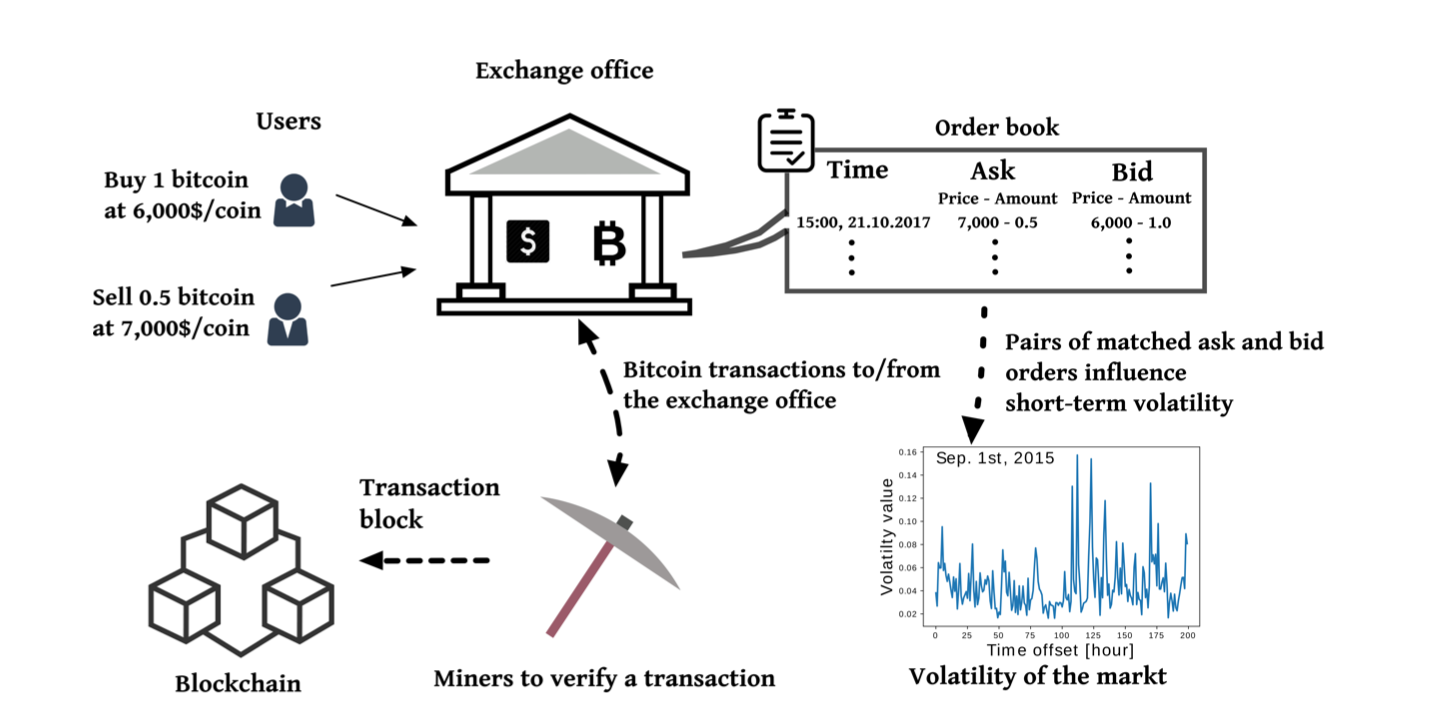
\includegraphics[width=0.6 \textwidth]{images/mine}
	\centering
	\caption{روند کلی استخراج و نحوه‌ی کار رمز‌ارزها \cite{guo2018bitcoin}.
	}
	\label{fig.panjda}
\end{figure}

\subsection{دفتر سفارشات}
دفتر سفارشات داده ساختاریست که نگهدارنده‌ي وضعیت فعلی بازار و سفارشات خریداران و فروشندگان است. هر سفارش خرید\LTRfootnote{bid} شامل دو عدد حجم و قیمت است، که بیان کننده‌ی تقاضای خرید به مقدار حجم مشخص‌شده از آن دارایی در قیمتی کمتر یا مساوی با قیمت مشخص شده‌اند. در مقابل هر تقاضای فروش\LTRfootnote{ask} نیز نشان دهنده‌ی تقاضای فروش به مقدار حجم مشخص‌شده از آن دارایی در قیمتی بیشتر و یا مساوی با قیمت مشخص شده است. معامله و جابه‌جایی دارایی تنها هنگامی صورت می‌گیرد که قیمت پیشنهادی خریدار بیشتر و یا مساوی با قیمت پیشنهادی فروشنده باشد، در چنین شرایطی به میزان حجم مشخص شده از دارایی فروشنده به دارایی خریدار انتقال صورت می‌گیرد و هر دو سفارش از دفتر سفارشات خارج می‌شوند.
\begin{figure}[!t]
	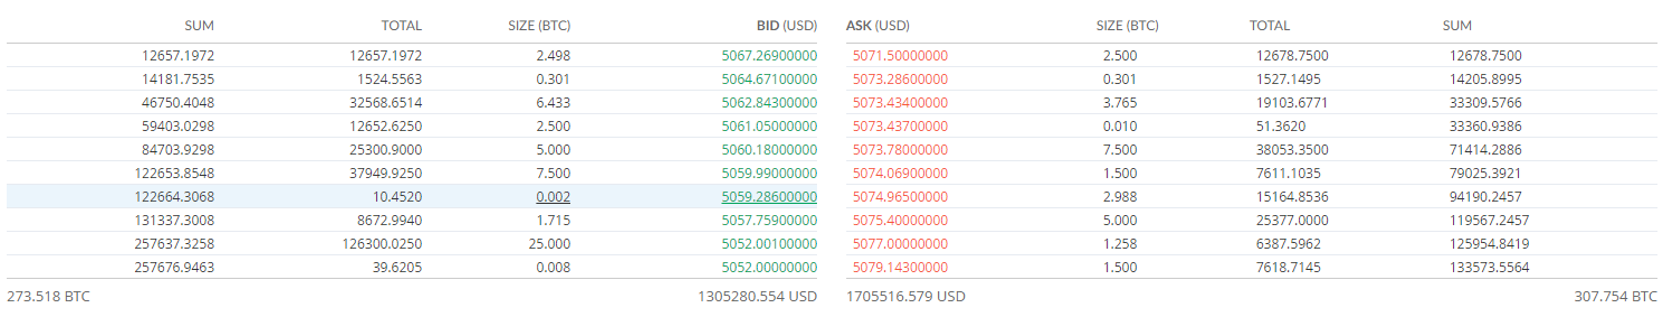
\includegraphics[width=1.0 \textwidth]{images/orderbook}
	\centering
	\caption{ نمونه‌ای از دفتر سفارشات مربوط به بیتکوین.
	}
	\label{fig.panda}
\end{figure}
\subsection{نوسان قیمت در رمزارزها}
به دلیل استقبال گسترده از رمزارزها در سال‌های گذشته، مطالعات زیادی بر روی ویژگی‌های آماری بازار رمزارز‌های مختلف انجام شده است. یکی از زمینه‌های اصلی این مطالعات نوسان قیمت در این بازارها بوده‌است. بر خلاف افزایش اندازه بازار رمزارز‌ها، این بازارها همچنان دارای نوسان بسیار زیادی نسبت به بازار‌های هم اندازه‌ هستند که محل بررسی بوده است\cite{katsiampa2017volatility}. برخی این میزان از نوسان را به دلیل عدم وجود روش دقیقی برای ارزش‌گذاری این ارزها که مورد پذیرش همگان باشد می‌دانند. این مسئله موجب شده است تا مطالعات مختلفی به بررسی این ویژگی این بازارها بپردازند.
\section{راه حل پیشنهادي}
در این پروژه، سعی داریم تا با استفاده از اطلاعات موجود در دفتر سفارشات یک مدل نوسانی بر پایه یادگیری عمیق ارائه بدهیم. مطالعات مختلفی نشان دهنده‌ی اهمیت و تاثیر دفتر سفارشات بر متغیر‌های مختلف بازارها بوده‌اند. در مقایسه با دیگر منابع داده‌ی موجود، دفتر سفارشات حجیم‌تر است و شامل اطلاعات جزئی‌تری از وضعیت فعلی بازار است. این اطلاعات که شامل سفارشات انجام نشده هستند تا حدودی خبر از آینده‌ی نزدیک بازار می‌دهند، و از این جهت در مقدار و جهت تغییرات بازار که همان نوسان است تاثیر قابل توجهی دارند\cite{guo2018bitcoin}و\cite{donier2015markets}.\\
از طرفی شبکه‌های عصبی در سال‌های گذشته در بسیاری از زمینه‌ها به صورت گسترده به کار گرفته شده‌اند و نتایج بسیار امیدوار کننده‌ای ارائه داده‌اند. با این وجود، شبکه‌های عصبی معمولی در استفاده از دنباله‌ی طولانی‌ای از داده‌های ورودی و یادگیری در چنین شرایطی مشکلات مختلفی دارند و کارا نیستند\cite{wang2015back}. در این میان، شبکه‌های عصبی بازگشتی\LTRfootnote{Recurrent Neural Network}، به کمک طراحی خود و استفاده از دنباله‌ای از اطلاعات ورودی برای پیش‌بینی اطلاعات آینده، عملکرد بهتری در این زمینه‌ ارائه کرده‌اند. هرچند که این مدل‌ها نیز در یافتن و استفاده از اطلاعات بلندمدت در دنباله‌ی طولانی از اطلاعات ناتوانند. شبکه‌های بازگشتی معمولی در مواجهه با دنباله‌ی طولانی از اطلاعات ،به ویژه در مسائل سری‌های زمانی، با مشکل ناپدید شدن گرادیان\LTRfootnote{Vanishing Gradient Problem} مواجه می‌شوند\cite{hochreiter1998vanishing}و\cite{pascanu2013difficulty}. به طور دقیق‌تر گرادیان بعد از طی کردن مسیر طولانی مقدار بسیار کمی اتخاذ می‌کند که باعث مشکل در روند یادگیری می‌شود. در چنین شرایطی مدل تنها حافظه‌ی کوتاه مدت دارد و توانایی استفاده از روابط طولانی‌مدت‌تر را نخواهد داشت.\\
برای رفع این مشکل شبکه‌های حافظه طولانی کوتاه‌مدت\LTRfootnote{Long short-term memory} ارائه شده‌اند\cite{hochreiter1997long}. این شبکه‌ها با استفاده از متغیرها و ارتباطات مخصوصی که برای حافظه در نظر گرفته‌اند، در طول انتشار معکوس\LTRfootnote{Back Propagation} مقادیر گرادین را تا حدودی حفظ می‌کنند و از ناپدید شدن آن جلوگیری می‌کنند. در این پروژه تصمیم داریم با استفاده از گونه‌ی دیگری از این ساختارهای اصلاح شده به نام جی‌آریو\LTRfootnote{Gated reccurent unit} و دنباله‌ای از اطلاعات استخراج شده از دفتر سفارشات، اقدام به پیش‌بینی سری زمانی نوسان در این بازار‌ها کنیم.
\section{بخش‌بندي پایان‌نامه}
در بخش بعدی،‌ کارهای مشابه و مربوط به پروژه‌ را بررسی می‌کنیم و مورد مطالعه قرار می‌دهیم. در میان کارهای مطالعه شده بعضا عمیق‌تر شده و به توضیح مدل‌های احتمالاتی برای پیش‌بینی نوسان می‌پردازیم. در بخش روش پیشنهادی،‌ نحوه‌ی استخراج ویژگی‌های مورد استفاده از دفتر سفارشات را توضیح خواهیم داد، و سپس به ارائه‌ی ساختار مدل پیشنهادی و نحوه‌ی آموزش خواهیم پرداخت. سپس در بخش پیاده‌سازی جزییات نحوه‌ی پیاده‌سازی، کتابخانه‌های استفاده شده و نحوه‌ی کار سیستم را توضیح خواهیم داد. بعد از آن در بخش ارزیابی به معرفی منابع داده‌ی استفاده‌شده و مقایسه‌ی روش‌های مختلف خواهیم پرداخت. در بخش پایانی نیز به بیان پیشنهادات برای کارهای آینده و جمع‌بندی نهایی خواهیم پرداخت.

%\chapter{پیش‌زمینه و کارهای مرتبط‌}
\section{مقدمه}
در این بخش، ابتدا به تبیین مفهوم نوسان و بیان مدل ریاضی آن از دیدگاه‌های متفاوت می‌پردازیم. سپس سعی می‌کنیم تا برخی از کارهای مرتبط در این حوزه را معرفی کنیم. از راهکارهای متفاوتی برای پیش‌بینی‌ سری‌های زمانی مختلف و همچنین نوسان همان سری‌های زمانی استفاده شده است که در ادامه به مطالعه‌ی برخی از ‌آنها خواهیم پرداخت.\\
هرچند به صورت سنتی اکثر مدل‌هاي مربوط به محاسبه‌ي نوسان آماري هستند، فعالیت‌هاي تحقیقاتی متعددي در این زمینه در سالهاي گذشته انجام شده است که دامنه وسیعی از ابزارهاي حوزه هوش مصنوعی را به کار گرفته‌اند. دامنه مجموعه داده‌ي مورد استفاده در این کارها نیز گوناگون است، درحالی که برخی تنها از اطلاعات قیمت و حجم مورد مبادله استفاده می‌کنند، برخی دیگر پا را فراتر گذاشته و از اطلاعات دفتر سفارشات نیز استفاده می‌کنند. برخی دیگر با استفاده از داده‌هاي با فرکانس بسیار بالا و در حد چند میلی‌ثانیه سعی در تخمین وضعیت بازار در بازه‌ی زمانی کوتاهی در آینده را با دقتی بالاتر از حد معمول دارند که در معاملات با فرکانس بالا\LTRfootnote{High-frequency trading} کاربرد دارد. اما تلاش اصلی همواره در جهت به دست آوردن تخمینی از وضعیت بازار در چند دقیقه‌ی آینده در یک بازار مالی بوده‌است.\\
مدل‌های یادگیری عمیق و به ویژه مدل‌های شبکه‌ی عصبی بازگشتی نیز در سال‌های گذشته در زمینه‌ی پیش‌بینی سری‌های زمانی بیشتر به کار گرفته شدند و حتی برخی مطالعات از پیشتازی این روش‌ها در برخی کاربردها خبر می‌دهند.
% از میان این مدل‌ها نیز به معرفی چندگونه خواهیم پرداخت و نحوه‌ی عملکرد ‌آن‌ها را مورد بررسی قرار خواهیم داد.

\section{نوسان} 
در این بخش ابتدا نوسان را به صورت دقیق تعریف می‌کنیم و سپس به مطالعه‌ی تعدادی از مدل‌های نوسانی معروف و نحوه‌ی عملکرد آن‌ها می‌پردازیم.
\subsection{تعریف نوسان}
ابتدا به معرفی نماد‌های مورد استفاده برای تعریف نوسان می‌پردازیم. $P_t$ را قیمت یک دارایی در لحظه‌ی $t$ در نظر می‌گیریم. بازده\LTRfootnote{Return} در لحظه‌ی $t$ به معنای سود یا ضرریست که دارایی مورد نظر در آن لحظه‌ تجربه ‌می‌کند. بر پایه‌ی $P_t$ بازده در لحظه‌ي $t$ به صورت زیر تعریف می‌شود:
\begin{equation}
	\label{eq:t}
	r_t = ln(P_t) - ln(P_{t-1})
\end{equation}
بر این اساس، میانگین بازده در یک پنجره‌ی $N$تایی به صورت زیر تعریف می‌شود:
\begin{equation}
	\label{eq:t1}
		\bar{r}_t = \dfrac{\Sigma_{i=0}^{N-1} r_{t-i}}{N}
\end{equation}
به همین شکل واریانس تغییرات قیمت برای پنجره‌ای به طول $N$، که به عنوان نوسان شناخته می‌شود،‌ به صورت زیر محاسبه می‌شود:
\begin{equation}
	\label{eq:vol}
	v_t = \sqrt{\dfrac{\Sigma_{i=0}^{N-1} (r_{t-i}-\bar{r})^2}{N}}
\end{equation}
طبق رابطه‌ی بالا می‌توان سری زمانی نوسان، $v_t$ را در طول زمان تشکیل داد.
\section{مدل‌های نوسانی}
در ادامه به معرفی ویژگی‌های مدل‌های نوسانی مختلف و بررسی نحوه‌ی کارکرد برخی از آن‌ها می‌پردازیم. مطالعات پیشین به استفاده و بررسی گسترده از مدل‌های بر پایه‌ی مدل گارچ\LTRfootnote{GARCH} برای پیش‌بینی نوسان پرداخته اند\cite{katsiampa2017volatility}و\cite{liu2019volatility}. برخی دیگر از روش‌های مبتنی بر مدل‌های احتمالاتی گرافی برای استفاده از اطلاعات موجود در دفتر سفارشات استفاده کرده‌اند\cite{guo2018bitcoin}.\\
\subsection{مدل‌های گارچ}
برای درک نحوه‌ی کارکرد مدل‌های گارچ ابتدا باید از گونه‌ی ساده تری از مدل ها به نام آریما\LTRfootnote{Arima} که خود شامل سه بخش کاهنده‌ی خودکار\LTRfootnote{Auto Regressive}، میانگین متحرک\LTRfootnote{Moving Average} و بخش تجمعی\LTRfootnote{Integrated} هستند شروع کنیم.
\subsubsection{مدل‌های کاهنده‌ی خودکار}
$AR(p)$ یک مدل کاهنده‌ی خودکار از مرتبه‌ی $p$ است که از پس‌افت‌های\LTRfootnote{Lag} سری زمانی اصلی به عنوان متغیرهای پیش‌بینی همان سری زمانی در آینده استفاده می‌کند. مقدار $p$  بیان کننده‌ی مرتبه‌ی مدل است. به عنوان مثال، $AR(1)$ از پس‌افت اول سری زمانی، یعنی $x_{t-1}$، برای پیش بینی $x_t$ استفاده می‌کند. بنابراین می‌توان  یک مدل کاهنده‌ی خودکار  از مرتبه‌ی $p$را به صورت زیر تعریف کرد\cite{ariyo2014stock}:
\begin{equation}
	x_t = \phi_0 + \phi_1 x_{t-1} + \phi_2 x_{t-2} + ... + \phi_p x_{t-p} + \epsilon_t
\end{equation}
که $\epsilon_t$ در آن نویز سفید\LTRfootnote{White Noise} است. در واقع $\epsilon$ هربار بعد از مشاهده‌ی مقدار اصلی سری زمانی به صورت اختلاف پیش‌بینی مدل و مقدار اصلی محاسبه می‌شود. $\epsilon$ در حالت ایده‌آل نویز سفید است، چرا که در این صورت می‌توانیم مطمئن باشیم که مدل تمامی الگوهای موجود در سری زمانی را مدل کرده است و مقدار باقیمانده\LTRfootnote{Residual Value} از سری‌زمانی کاملا تصادفی و غیرقابل مدل کردن است.

\subsubsection{مدل‌های میانگین متحرک}
این مدل‌‌ها از جهاتی به مدل‌های کاهنده‌ی خودکار شبیه هستند، اما به جای استفاده از پس‌افت‌های قبلی سری زمانی،‌ از خطاها($\epsilon$) برای پیش‌بینی استفاده می‌کنند. مدل‌ $MA(q)$ یک مدل‌ میانگین متحرک از مرتبه‌ی $q$ است که از تعداد $q$ خطای قبلی برای پیش‌بینی سری زمانی استفاده می‌کند، که به صورت زیر تعریف می‌شود:
\begin{equation}
	x_t = \epsilon_t + \theta_1 \epsilon_{t-1} + \theta_2 \epsilon_{t-2} + ... + \theta_q \epsilon_{t-q} + \mu
\end{equation}
که $\mu$ بیانگر میانگین ثابت است.
\subsubsection{مدل‌های آریما}
این مدل‌های که به نوعی ترکیب دو مدل قبلی هستند، از تمامی ویژگی‌های موجود در آن‌ها بهره می‌برند. این مدل‌ها ابتدا متغیر جدید $y_t$ را به صورت زیر تعریف می‌کنند:
\begin{equation}
	\label{eq:airami}
	y_t = x_t - x_{t-1}
\end{equation}
علت تعریف $y_t$  به این صورت از بین بردن رشد خطی یک سری زمانی یا روند سیر\LTRfootnote{Trend} آن است. بدیهی است که در صورت توانایی پیش‌بینی سری‌زمانی $y$ می‌توان به راحتی سری زمانی $x$ را با داشتن یک مقدار اولیه به دست آورد. مدل آریما سری زمانی $y_t$ را به صورت زیر مدل می‌کند:
\begin{equation}
	\label{eq:arimapq}
	y_t = \phi_0 + \phi_1 x_{t-1} + ... + \phi_p x{t-p} + \epsilon_t + \theta_1 \epsilon_{t-1} + ... + \theta_q \epsilon_{t-q}
\end{equation}
که مانند مدل‌های قبلی مقادیر $p$ و $q$ مرتبه‌ی مدل آریما را مشخص می‌کنند. $p$ مرتبه‌ی قسمت کاهنده‌ی خودکار و $q$ مرتبه‌ی قسمت میانگین متحرک است. مدل‌ پارامتر دیگری به نام $i$ نیز دارد که عموما مقدار ۱ دارد اما بسته به کاربرد ممکن است تغییر کند و مقداری بیشتر از ۱ بگیرد. $i$ در مدل آریما مشخص می‌کند که عمل تفاضل‌گیری از سیگنال اولیه چندبار انجام شود. به عنوان مثال، رابطه‌ی \ref{eq:airami} نشان‌دهنده‌ی یکبار تفاضل‌گیری از سیگنال اولیه است. در صورتی که $i$ مقداری بیشتر از یک داشته باشد، باید عمل تفاضل‌گیری برای $y_t$ نیز تکرار شود تا سری زمانی جدید تشکیل شود و سپس از رابطه‌ی \ref{eq:arimapq} برای مدل‌کردن آن استفاده شود.
\subsubsection{مدل‌های آرچ}
مدل‌های بر پایه‌ی آرچ\LTRfootnote{Autoregressive conditional heteroskedasticity} با تمرکز بر پیش‌بینی نوسان به وجود آمده‌اند. این مدل میزان نوسان هر نقطه‌ی زمانی را با استفاده از خطای پیش‌بینی در نقاط قبل از آن یعنی $\epsilon$ها مدل‌ می‌کند. این مدل نیز مانند مدل‌های پیشین برای پایه‌های مختلف تعریف می‌شود. تعریف یک مدل آرچ به ازای پایه‌ی $r$ برابرست با:
\begin{equation}
	\epsilon_t = w_t \sqrt{\alpha_0 + \alpha_1 \epsilon_{t-1}^2 + \alpha_2 \epsilon_{t-2}^2 + ... + \alpha_r \epsilon_{t-r}^2}
\end{equation}
که در حالت ایده‌آل، $w_t$ در آن باید نویز سفید باشد که بعد از مشاهده‌ی مقدار اصلی نوسان دنباله‌ی هدف قابل محاسبه می‌باشد.
\subsubsection{مدل‌های گارچ}
نحوه‌ی بدست آمدن مدل‌ گارچ از روی مدل‌ آرچ بسیار شبیه به روند تبدیل مدل‌ کاهشی خودکار به آریماست. در تبدیل مدل کاهشی خودکار به آریما شاهد بودیم که با اضافه کردن یک مجموعه متغیر جدید که نشان‌دهنده‌ی خطای پیش‌بینی‌های گذشته بودند، مدل‌ کامل‌تری ساخته شد که می‌توانست از خطاهای قبلی خود در جهت بهبود پیش‌بینی‌های بعدی استفاده کند. در تبدیل آرچ به گارچ نیز با اضافه کردن پس‌افت‌های خود سری زمانی نوسان به مدل قبلی،‌ می‌توانیم دنباله‌های بیشتری را مدل کنیم. رابطه‌ی گارچ برای پایه‌های $p$ و $q$ به صورت زیر است:
\begin{equation}
	\label{garch:one}
	\epsilon_t = w_t \sqrt{\alpha_0 + \alpha_1 \epsilon_{t-1}^2 + ... + \alpha_p \epsilon_{t-p}^2 + \beta_1 \delta_{t-1}^2 + ... + \beta_q \delta_{t-q}^2}
\end{equation}
در تعریف بالا $\delta_{t}$ به معنای نوسان در لحظه‌ی $t$ است که به صورت زیر قابل محاسبه است:
\begin{equation}
	\label{garch:twol}
	\delta_t = \sqrt{\alpha_0 + \alpha_1 \epsilon_{t-1}^2 + \alpha_2 \epsilon_{t-2}^2 + ... + \alpha_q \epsilon_{t-q}^2}
\end{equation}
با استفاده از \ref{garch:one} و \ref{garch:twol} می‌توان رابطه‌ی گارچ را به صورت زیر بازنویسی کرد:
\begin{equation}
	\epsilon_t = w_t \sqrt{\delta_{t} + \beta_1 \delta_{t-1}^2 + ... + \beta_q \delta{t-q}^2}
\end{equation}
که مانند مدل‌های قبلی $w_t$ نویز سفید است.
\subsection{دفتر سفارشات}
در این بخش به مطالعه‌ی بخشی از مطالعات انجام شده بر روی اطلاعات دفتر سفارشات خواهیم پرداخت. ابتدا به معرفی ساختار دفتر سفارشات خواهیم پرداخت و سپس مشاهده‌ خواهیم کرد که این داده ساختار چگونه اطلاعات مربوط به وضعیت بازار و سفارشات را در خود جای می‌دهد. در ادامه به بررسی چند نمونه از مطالعات انجام شده بر روی دفتر سفارشات خواهیم پرداخت و با اهمیت این داده ساختار در مطالعه‌ی بازارهای مالی آشنا خواهیم شد.
\begin{figure}[!t]
	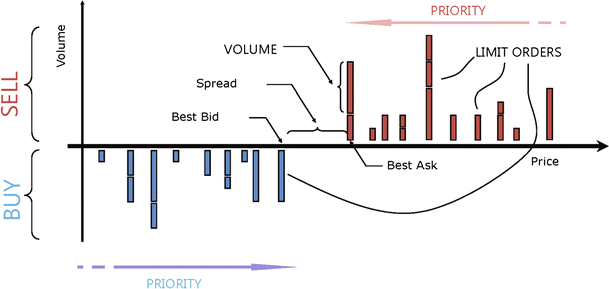
\includegraphics[width=1.0 \textwidth]{images/orderbook_1}
	\centering
	\caption{ نمودار ساختار دفتر سفارشات به همراه برخی ویژگی‌های مربوط\cite{brabazon2016characterising}.
	}
	\label{fig.orderbook_1}
\end{figure}

\subsubsection{ساختار دفتر سفارشات}
به طور خلاصه دفتر سفارشات شامل تمامی سفارش‌های خرید و فروش در جریان در یک بازار مالی و مربوط به یک دارایی مشخص است. این دفتر شامل سفارشات به صورت یک دوتایی مرتب شامل قیمت و حجم متناظر است. تمام سفارش‌هایی که دارای قیمت یکسانی باشند با یکدیگر تجمیع می‌شوند و به صورت یک دوتایی مرتب با همان قیمت و مجموع حجم همه‌ی آن‌ها در دفتر ثبت می‌شوند.\\
این دوتایی‌های مرتب را می‌توان بر اساس قیمت مرتب کرد تا بتوان ترتیبی برای نحوه‌ی جور کردن آن‌ها در جریان فعالیت بازار در نظر گرفت. در صورت مرتب‌سازی این دوتایی‌ها بر اساس قیمت، مانند شکل \ref{fig.orderbook_1}، شاهد جداسازی سفارش های مربوط به خرید و سفارش‌های مربوط به فروش خواهیم بود. علت این امر آن است که سفارش‌های خرید همواره قیمت کمتری نسبت به قیمت سفارش‌های موجود برای فروش دارند، زیرا که اگر چنین نبود سفارش خرید به محض ایجاد با یک سفارش فروش متناظر می‌شد و معامله‌ انجام می‌شد و هر دو سفارش از دفتر سفارشات خارج می‌شدند.\\
سپس در حالی که دوتایی‌ها بر اساس قیمت مرتب‌سازی شده‌اند می‌توان یک ترتیب ‌برای نحوه‌ی جورسازی و اجرای آن‌ها در نظر گرفت. سفارش‌های فروش به ترتیب از قیمت کم به زیاد دارای اولویت زیاد به کم هستند چرا که خریداران همواره تمایل به خرید یک دارایی با کمترین قیمت ممکن را دارند و در نتیجه اگر قیمت پیشنهادیشان بیشتر از چند سفارش فروش مختلف باشد،‌ اقدام به خرید از ارزان‌ترین آن‌ها می‌کنند. برعکس همین مسئله برای سفارش‌های خرید برقرار است. بدین ترتیب سفارشی که بیشترین میزان قیمت پیشنهادی را داشته باشد از بالاترین اولویت برخوردار است و در صورتی که سفارش فروش جدیدی با قیمتی کمتر از چند سفارش خرید موجود در بازار ایجاد شود،‌ به طور خودکار با گران‌ترین سفارش خرید جور شده و اجرا می‌شود.\\
از طرف دیگر ویژگی‌های دیگری نیز در دفتر سفارشات وجود دارد که مورد علاقه‌ی تحلیلگران و فعالین این حوزه بوده است. از مهم ترین آن‌ها می‌توان به شکاف قیمت\LTRfootnote{Spread} که در شکل \ref{fig.orderbook_1} نیز مشاهده می‌شود اشاره کرد. شکاف قیمت بیانگر اختلاف موجود بین ارزان‌ترین پیشنهاد فروش و گران‌ترین پیشنهاد خرید است. به طور معمول افزایش میزان شکاف قیمتی خبر از اختلاف میان خریداران و فروشندگان می‌دهد که می‌تواند باعث افزایش یا کاهش شدید قیمت در آینده‌ی نزدیک بشود که در هر دو حالت با افزایش نوسان همراه خواهد بود.\\
در مطالعه‌ای نشان داده شده است که با استفاده از ویژگی‌های مختلف دفتر سفارشات می‌توان نوسان را با دقت بیشتری نسبت به روش‌هایی که ازین اطلاعات استفاده نمی‌کنند تخمین زد\cite{guo2018bitcoin}. این مقاله با استفاده از یک مدل احتمالاتی گرافی و اطلاعات دفتر سفارشات، موفق شده است که نوسان را با دقت بیشتری نسبت به مدل‌های گارچ پیش‌بینی کند. همچنین نکته‌ی دیگری که در این مقاله‌ حائز اهمیت است، مقایسه‌ی نتایج نهایی به دست آمده توسط این مدل با مدل‌های ساده‌ی شبکه‌ی عصبی است که نشان دهنده‌ی برتری شبکه‌های عصبی در برخی بازه‌های زمانی نیز هست.
\subsection{جمع بندی}
در این فصل با برخی روش‌های آماری برای پیش‌بینی سری‌های زمانی و نوسان آن‌ها آشنا شدیم. سپس به بررسی و معرفی دقیق‌تر دفتر سفارشات پرداختیم.
% و در انتها با روش‌های مبتی بر شبکه‌های عصبی برای محاسبه‌ی سری‌های زمانی آشنا شدیم.



%\chapter{روش پیشنهادی}
%\thispagestyle{empty}

\section{مقدمه}
در بخش قبلی با برخی پیشنیاز‌های مربوط به مسئله اصلی و برخی از مطالعات انجام شده در استفاده از دفتر سفارشات آشنا شدیم. در این بخش قصد داریم تا روش پیشنهادی برای حل مسئله را تشریح کنیم. ابتدا به نحوه‌ی ذخیره‌سازی و استخراج ویژگی‌های مختلف از دفتر سفارشات می‌پردازیم، سپس به سراغ تشکیل سری زمانی نوسان قیمت و ایجاد نمونه‌های برچسب دار می‌رویم. در ادامه با مدل‌های شبکه‌ی عصبی بازگشتی و به ویژه جی‌آریو آشنا می‌شویم و با استفاده از آن‌ها مدل نوسانی خود را تشکیل می‌دهیم.

\begin{figure}[!t]
	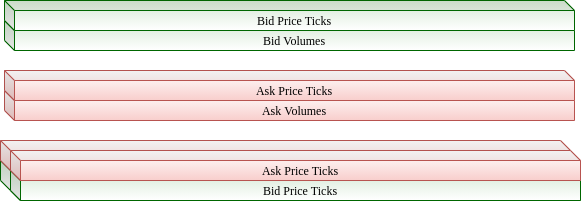
\includegraphics[width=1.0 \textwidth]{images/orderbook_structure}
	\centering
	\caption{نحوه‌ی جداسازی و ذخیره‌ی دفتر سفارشات	}
	\label{fig.orderbook_structure}
\end{figure}

\section{استخراج ویژگی و سری‌زمانی از دفتر سفارشات}
همانطور که در فصل قبل اشاره کردیم دفتر سفارشات را می‌توان به صورت دنباله‌ای از دوتایی‌های مرتب شامل قیمت و حجم متناظر در نظر گرفت. با جدا سازی دو بخش خرید و فروش و همچنین جداسازی دو بخش قیمت و حجم برای هر دفتر ثبت سفارش در طول زمان به یک آرایه‌ی سه بعدی که شامل تمامی اطلاعات دفتر سفارشات اولیه است دست پیدا می‌کنیم(شکل \ref{fig.orderbook_structure}). در این شکل آرایه‌ی سه بعدی مد نظر با ابعاد $2 * 2 * Depth$ نمایش داده شده است که $Depth$ یا عمق در آن به معنای تعداد سفارش‌های موجود در هر سمت دفتر سفارشات است. در این پروژه عمق دفتر سفارشات در هر دو سمت خرید و فروش را برابر در نظر می‌گیریم تا نمایش بهتری از داده‌ها داشته باشیم. هر دندانه‌ی\LTRfootnote{Tick} قیمتی به یک قیمت مشخص برای دارایی مورد مطالعه اشاره می‌کند. فواصل این دندانه‌ها توسط صرافی مربوطه تعیین می‌شود و گاها نسبت ثابتی با آخرین قیمت معامله‌شده دارد، اما عمدتا این فواصل به صورت ثابت و پیش‌فرض برابر مقدار کمی مانند ۱۰ سنت در نظر گرفته می‌شوند. علت این امر ایجاد انعطاف بیشتر برای خریداران و فروشندگان در سفارشات است. 

\subsection{دفتر سفارشات تجمعی}
در مرحله‌ی بعدی دفتر سفارشات تجمعی را تعریف می‌کنیم. هدف‌ اصلی از تعریف دفتر سفارشات تجمعی دستیابی به نمایش بهتری از عرضه و تقاضا نسبت به دفتر سفارشات عادی است\cite{blazejewski2004application}.\\
\begin{figure}[!t]
	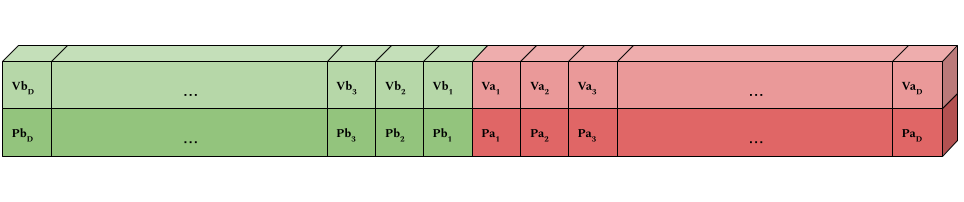
\includegraphics[width=1 \textwidth]{images/orderbook_t1}
	\centering
	\caption{اندیس گذاری دفتر سفارشات برای ایجاد دفتر سفارشات تجمعی	}
	\label{fig.orderbook_t1}
\end{figure}
حجم‌های تجمعی را بر اساس حجم‌های اولیه (شکل \ref{fig.orderbook_t1}) تعریف می‌کنیم:
\begin{equation}
	\begin{aligned}
			\bar{V}b_i = \sum_{j=1}^{i} Vb_j\\
			\bar{V}a_i = \sum_{j=1}^{i} Va_j
	\end{aligned}
\end{equation}
که $Vb_i$ و $\bar{V}b_i$ در آن به ترتیب بیانگر حجم خرید در دندانه‌ی $i$ام خرید و حجم تجمعی خرید در دندانه‌ی $i$ام هستند. به همین شکل، $Va_i$ و $\bar{V}a_i$ در آن به ترتیب بیانگر حجم فروش در دندانه‌ی $i$ام فروش و حجم تجمعی فروش در دندانه‌ی $i$ام هستند.\\
با تشکیل این دنباله‌های جدید، می‌توان تفسیر جدیدی برای دفتر سفارشات در نظر گرفت. در این نمایش جدید $\bar{V}$ها نشان دهنده‌ی حداکثر میزان حجم موجود برای خرید (یا فروش) در صورت تمایل به پرداخت (یا دریافت) قیمت متناظر با هر دندانه‌ هستند. بدین شکل هر دندانه‌ی سفارشی معنا‌ی کامل‌تری نسبت به حالت قبلی پیدا می‌کند چرا که محل قرارگیری سفارش‌های خریداران و فروشندگان در دفتر سفارشات در این نمایش جدید گنجانده شده‌است.\\
به طور مثال، قرار دادن یک سفارش خرید با حجم بسیار زیاد در نزدیکی بالاترین قیمت پیشنهادی خرید تمامی پیشنهادهای با قیمت کمتر را تحت تاثیر قرار می‌دهد و از احتمال اجرا شدن آن‌ها می‌کاهد. اینگونه سفارشات با حجم بالا که به عنوان دیوار قیمتی\LTRfootnote{Price Wall} شناخته می‌شوند از اهمیت بسیار زیادی برخوردار هستند چرا که وجود یا عدم وجودشان باعث تفسیر متفاوتی از سفارش‌های بعد از آنها می‌شوند.
\begin{figure}[!t]
	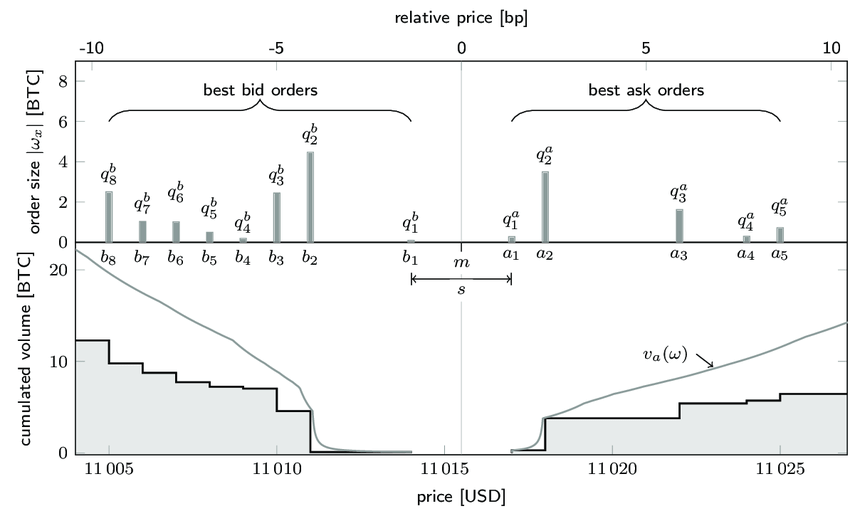
\includegraphics[width=1 \textwidth]{images/orderbook_t2}
	\centering
	\caption{نمونه‌ای از دفتر سفارشات معمولی و دفتر سفارشات تجمعی متناظر\cite{Schnaubelt2019}}
	\label{fig.orderbook_t2}
\end{figure}
\subsection{استخراج ویژگی‌های دیگر از دفتر سفارشات}
در این مرحله به استخراج برخی دیگر از ویژگی‌های دفتر سفارشات که در برخی از مطالعات انجام‌شده بر روی دفتر سفارشات از آن‌ها استفاده شده‌است می‌پردازیم.
\subsubsection{قیمت میانی}
قیمت میانی برای هر دفتر سفارشات به صورت میانگین بیشترین قیمت خرید و کمترین قیمت فروش در نظر گرفته می‌شود. این مقدار را به صورت زیر می‌توان تعریف کرد:
\begin{equation}
	MidPrice = \dfrac{(Pb_1 + Pa_1)}{2} 
\end{equation}
قیمت میانی می‌تواند تخمین خوبی از قیمتی که معامله‌ی بعدی در آن انجام می‌شود به دست دهد و از این جهت حائز اهمیت است.
\subsubsection{شکاف قیمت}
شکاف قیمت\LTRfootnote{Price Spread} اختلاف بین بالاترین قیمت خرید و پایین‌ترین قیمت فروش است. که به صورت زیر محاسبه می‌شود:
\begin{equation}
	PriceSpread = Pa_1 - Pb_1 
\end{equation}

\subsubsection{تغییر قیمت یا بازده}
مقدار تغییر قیمت که به آن بازده نیز گفته می‌شود، معمولا به صورت لگاریتمی در مطالعات استفاده می‌شود. این مقدار با استفاده از دو قیمت میانی متوالی قابل محاسبه است که به صورت مقابل نشان داده می‌شود:
\begin{equation}
	PriceChange_{t+1} = ln(\dfrac{MidPrice_{t+1}}{MidPrice_t}) = ln(MidPrice_{t+1})  - ln(MidPrice_t)
\end{equation}

\subsubsection{شکاف قیمتی وزن‌دار}
این مقدار بیانگر اختلاف موجود میان مجموع تقاضای خرید و فروش است. برای محاسبه‌ی این مقدار به طور معمول از ۱۰\% اول دفتر سفارشات استفاده می‌کنیم تا یک میانگین وزن‌دار از مجموع تقاضاهای خرید و فروش موجود در این بازه بسازیم. این مقدار را به صورت مقابل تعریف می‌کنیم:
\begin{equation}
	WheigtedSpread = \dfrac{1}{n}(\sum_{i=1}^{n}Pa_i * Va_i - \sum_{i=1}^{n}Pb_i * Vb_i)
\end{equation}
\vspace{-2em}
$$
	n = Depth / 10
$$
\newpage
\subsubsection{نوسان}
نوسان قیمت را نیز طبق فرمول \ref{eq:vol} برای پنجره‌های مختلف استخراج می‌کنیم و به مجموعه‌ داده ورودی برای هر نقطه اضافه می‌کنیم.
\subsection{استانداردسازی ویژگی‌ها}
در ادامه برای یادگیری بهتر لازم است تا ویژگی‌های استخراج‌شده را از نظر آماری استاندارد کنیم. یک ویژگی استاندارد داری میانگین صفر و واریانس یک است،‌ و برای استانداردسازی هر ویژگی باید ابتدا میانگین مقدار آن و انحراف معیار آن را در طول زمان را به دست بیاوریم و سپس طبق رابطه‌ی زیر ویژگی را استاندارد کنیم:
\begin{equation}
	X_{standard} = \dfrac{X - \bar{X}}{\delta}
\end{equation}
که $X$ بیانگر مقدار ویژگی در هر نقطه، $\bar{X}$ میانگین ویژگی $X$ در طول زمان و $\delta$ برابر انحراف معیار ویژگی $X$ است.
\section{یادگیری}
در این پروژه قصد داریم تا با استفاده از مدل‌های شبکه‌ی عصبی بازگشتی اقدام به یادگیری توزیع نوسان بر حسب ویژگی‌های استخراج شده کنیم. در این راستا، ابتدا شبکه‌های بازگشتی عمیق ساده را معرفی می‌کنیم و مشکلات آن‌ها را بررسی می‌کنیم. سپس به ساختار مدل جی‌آریو می‌پردازیم و راه حل این مدل برای مشکلات گفته شده را بررسی می‌کنیم. در انتها نحوه‌ی یادگیری بر اساس نمونه‌ها توسط این مدل را تشریح می‌کنیم.
\subsection{شبکه‌های عصبی بازگشتی}
شبکه‌های عصبی بازگشتی برای یادگیری داده‌هایی که طبیعت دنباله‌ای دارند طراحی شده‌اند\cite{weigend1990predicting}. این شبکه‌ها به دلیل ساختار دنباله‌ای در زمینه‌های مختلفی مانند پردازش زبان طبیعی و همچنین پیش‌بینی سری‌های زمانی به صورت گسترده استفاده شده‌اند.
\begin{figure}[!t]
	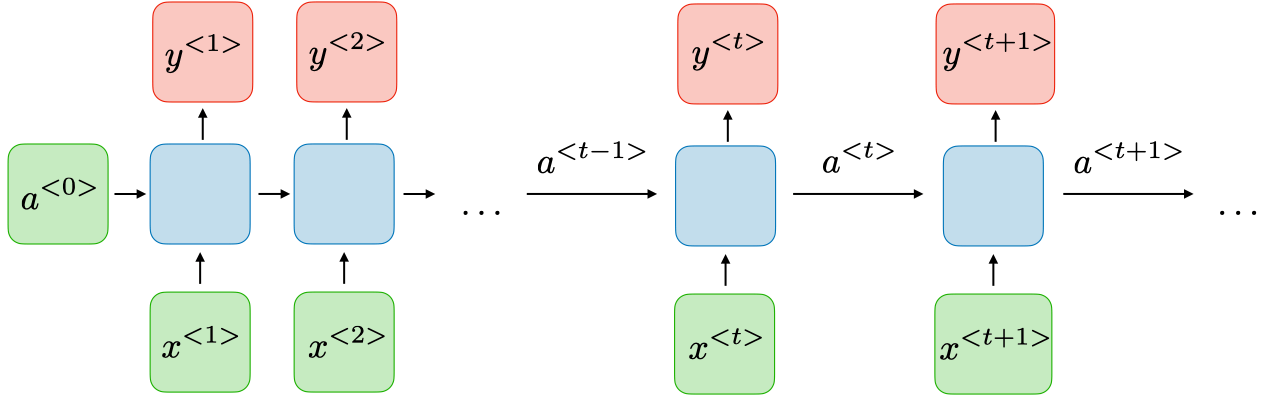
\includegraphics[width=1 \textwidth]{images/rnn_1}
	\centering
	\caption{شمای کلی شبکه‌های عصبی بازگشتی}
	\label{fig.rn1}
\end{figure}
این شبکه‌ها یک دنباله‌ی ورودی از داده‌ها را می‌گیرند و دنباله‌ای دیگر به عنوان خروجی تولید می‌کنند.\\
برای هر نقطه‌ی زمانی $t$، تابع فعال‌سازی $\alpha^{<t>}$ و تابع خروجی $y^{<t>}$ به صورت زیر محاسبه می‌شوند:
\begin{equation}
	\label{eq:rnn1}
	\alpha^{<t>} = g_1(W_{aa}\alpha^{<t-1>} + W_{ax}x^{<t>} + b_a)
\end{equation}
\vspace{-4em}
\begin{equation}
	\label{eq:rnn2}
	y^{<t>} = g_2(W_{ya}a^{<t>} + b_y)
\end{equation}
که ماتریس‌های $b_a$، $b_y$، $W_{ya}$، $W_{aa}$ و $W_{ax}$ در آن ضرایبی هستند که توسط هر سلول به اشتراک گذاشته می‌شود. از طرفی $g_1$ و $g_2$ نیز توابع فعال‌سازی\LTRfootnote{Activation Function} هستند که در ادامه با آن‌ها خواهیم پرداخت.
\begin{figure}[!t]
	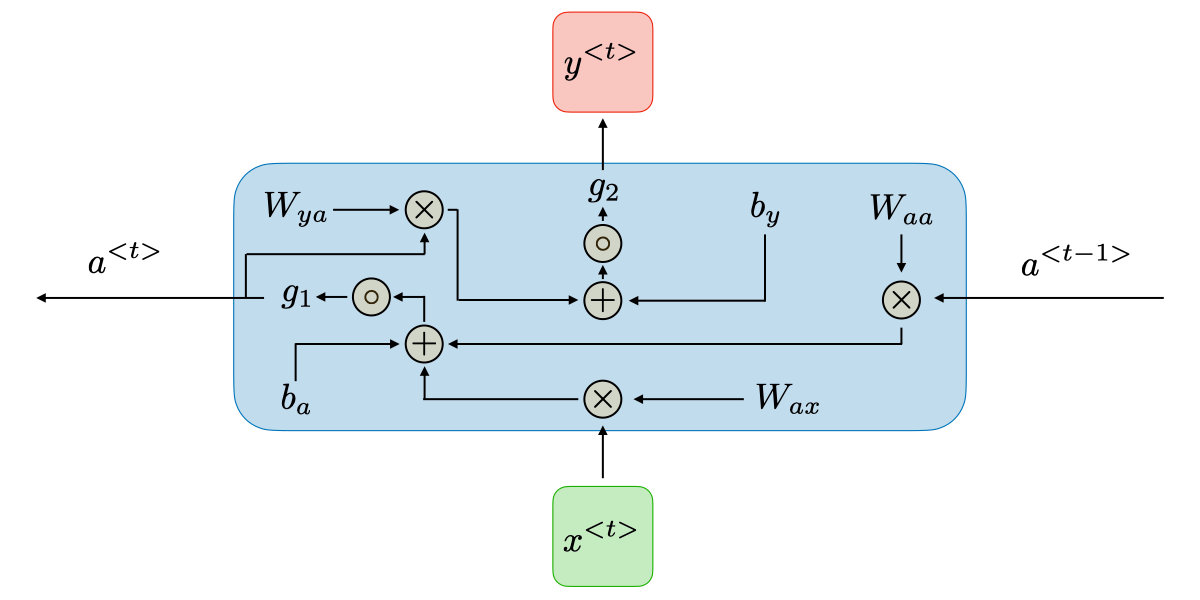
\includegraphics[width=0.8 \textwidth]{images/rnn_cell}
	\centering
	\caption{نمایی از روابط \ref{eq:rnn1} و \ref{eq:rnn2} که نحوه‌ی محاسبات انجام شده درون هر سلول شبکه‌ی عصبی بازگشتی را نشان می‌دهند.}
	\label{fig.rncell}
\end{figure}
\newpage
استفاده از شبکه‌های عصبی بازگشتی مزایا و معایب متفاوتی دارد که در ادامه به آن‌ها اشاره می‌کنیم.
\subsubsection{معایب شبکه‌های بازگشتی}
همانطور که پیش‌تر گفته شد. شبکه‌های عصبی بازگشتی از مشکل از بین رفتن گرادیان رنج می‌برند\cite{hochreiter1998vanishing}. این مسئله از تضعیف مقدار گرادیان در انتقال بین سلول‌ها ناشی می‌شود. هنگامی که فاصله‌ی نقطه‌ای که خطا در آن محاسبه شده با یک سلول زیاد می‌شود، گرادیان خطا نسبت به متغیرهای آن سلول مقدار بسیار کمی می‌گیرند که مانع از انجام یادگیری توسط مدل می‌شود. این مسئله باعث می‌شود تا ارتباطات بلندمدت در دنباله‌ی ورودی توسط مدل یاد گرفته نشود. در ادامه خواهیم دید که شبکه‌ی جی‌آریو چگونه با استفاده از حافظه‌ی داخلی این مشکل را برطرف می‌کند.\\
از طرف دیگر، به دلیل انتقال یک طرفه‌ی اطلاعات در این شبکه‌ها، امکان انتقال خطا از سلول‌های جلویی به عقبی وجود ندارد و به همین دلیل ورودی‌های بعدی در وضعیت فعلی متغیرهای سلول تاثیری نخواهند داشت. هرچند این مسئله در پیش‌بینی سری‌های زمانی خیلی مطرح نیست چرا که اغلب بر اساس دنباله‌ای از داده‌های ثبت شده در یک بازه‌ی زمانی به پیش‌بینی نقطه‌های بعدی می‌پردازیم. اما این مشکل در پردازش زبان طبیعی بسیار حائز اهمیت است که موجب پیدایش شبکه‌ها بر پایه توجه\LTRfootnote{Attention} شده‌است.
\subsubsection{مزایای شبکه‌های بازگشتی}
این شبکه‌ها به خاطر به اشتراک‌گذاری وزن‌ها در طول زمان، نسبت به افزایش طول ورودی حساسیتی ندارند و با افزایش طول ورودی تعداد پارامتر‌های آن‌ها افزایش نمیابد. این ویژگی این شبکه‌ها را برای استفاده در مسائل پیش‌بینی سری‌های زمانی که گاهی دارای ورودی بسیار بزرگ هستند مناسب می‌کند.\\
از طرفی، با به اشتراک‌گذاری وزن‌ها بین سلول‌ها، به نوعی دانش موجود برای نقاط مختلف زمانی به اشتراک گذاشته می‌شود، که باعث به وجود‌ آمدن مدل‌های کاراتری می‌شود. اطلاعات و خروجی توابع فعال‌سازی سلول‌های قبلی نیز در هر سلول به کار گرفته می‌شوند که ویژگی بسیار مناسبی در پیش‌بینی سری‌های زمانیست.\\
\newpage
\subsection{جی‌آریو}
جی‌آریو گونه‌ای از شبکه‌های عصبی بازگشتیست که برای حل مسئله‌ی گردایان از بین رونده و مدل‌سازی روابط طولانی مدت در داده‌های ورودی به وجود آمده است. این شبکه‌ها با استفاده از ساختاری مشابه به حافظه اقدام به حفظ اختیاری اطلاعات سلول‌های گذشته و انتقال آن‌ها به سلول‌های بعدی می‌کنند.\\
\begin{figure}[!t]
	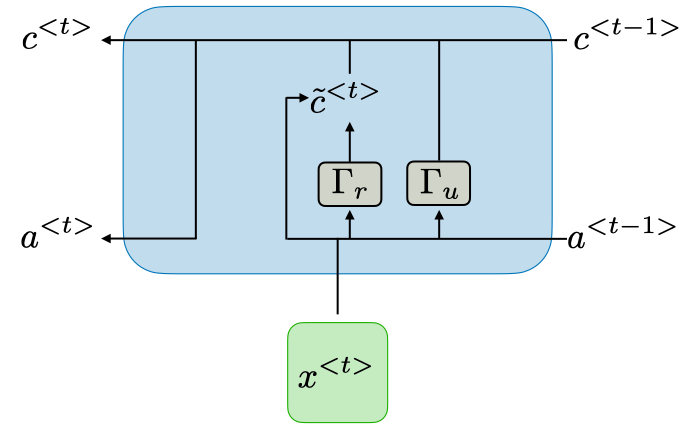
\includegraphics[width=0.8 \textwidth]{images/gru_1}
	\centering
	\caption{ساختار داخل هر سلول از شبکه‌ی عصبی جی‌آریو.}
	\label{fig.gru_1}
\end{figure}
برای متوجه شدن بهتر نحوه‌ی کارکرد این مدل از شبکه‌های عصبی روابط ریاضی آن‌ها را تشریح می‌کنیم:
\begin{equation}
	\tilde{c}^{<t>} = tanh(W_c[\Gamma_r * \alpha^{t-1} , x^{<t>}] + b_c)
\end{equation}
\vspace{-4em}
\begin{equation}
	\tilde{c}^{<t>} = tanh(W_c[\Gamma_r * \alpha^{t-1} , x^{<t>}] + b_c)
\end{equation}
\vspace{-4em}
\begin{equation}
	a^{<t>} = c^{<t>}
\end{equation}
که $\Gamma$ در آن مشخص کننده‌ی دروازه‌هاست که هرکدام هدف مشخصی دارند. رابطه ریاضی برای هر دروازه به صورت زیر است:
\begin{equation}
	\Gamma = \sigma(Wx^{<t>} +Ua^{<t-1>} + b)
\end{equation}
که $b$، $U$ و $W$ ضرایب متناظر با هر دروازه هستند و $\sigma$ تابع سیگموید است. که به صورت زیر تعریف می‌شود:
\begin{equation}
	\sigma(x) = \dfrac{1}{1 + e^{-x}}
\end{equation}
در هر سلول جی‌آریو $\Gamma_r$ مشخص کننده میزان ارتباط اطلاعات ورودی جدید در زمان $t$ است و به آن‌ دروازه‌ی ربط گفته می‌شود. این دروازه مشخص می‌کند که تا چه میزان اطلاعات ورودی جدید وارد حافظه‌ی بلندمدت یا همان متغیر $\tilde{c}$ بشود. از طرف دیگر، $\Gamma_u$ مشخص می‌کند که اطلاعاتی که از قبل درون حافظه وجود داشته اند تا چه میزان باید فراموش شوند و چه میزان از آن‌ها باید حفظ شود و ازین جهت به آن دروازه‌ی به‌روزرسانی گفته می‌شود.
\subsection{تابع خطا}
معیار‌های مختلفی برای گزارش خطا در پیش‌بینی سری‌های زمانی وجود دارد. تعریف تابع خطا در مطالعات بر روی سری زمانی اهمیت بسیار زیادی دارد، چرا که توابع خطا‌ی مختلف نتیجه‌های بسیار متفاوتی در مدل‌ نهایی به وجود می‌آورند. به طور مثال، توابع خطایی که با داده‌های پرت\LTRfootnote{Outlier} مانند باقی داده‌ها رفتار می‌کنند نتیجه‌ی قابل قبولی در مدل نهایی ارائه نمی‌دهند، چرا که این داده‌ها در سری‌های زمانی عموما غیر قابل پیش‌بینی هستند و به همین خاطر می‌توانند خطای قابل توجهی را به مدل‌ها تحمیل کنند. از طرف دیگر، هدف از به کار گیری مدل نوسان داشتن تخمین خوبی از نوسان در طول زمان به صورت عمومیست و نه فقط بازه‌های خاصی که پیش‌بینی ‌نوسان در آن‌ها بسیار سخت است،‌ به همین خاطر سعی در طراحی و استفاده از تابع خطا، جهت‌دهی یادگیری به سمتی است که در تعداد زیادی از نقاط تخمین خوبی از دنباله‌ی هدف توسط مدل حاصل شود. از همین جهت انواع مختلفی از توابع خطا در این حوزه به کار گرفته ‌شده‌اند که در ادامه به معرفی تعدادی از آن‌ها می‌پردازیم.
\newpage
\subsubsection{میانگین مربعات خطا}
این معیار خطا که به نوعی از نرم دوم خطا استفاده می‌کند،‌ با جمع زدن و میانگین‌گیری از مربعات خطا، معیاری از دقت عملکرد سیستم گزارش می‌دهد که رابطه‌ی آن به صورت زیر است:
\begin{align}
	\vcenter{\hbox{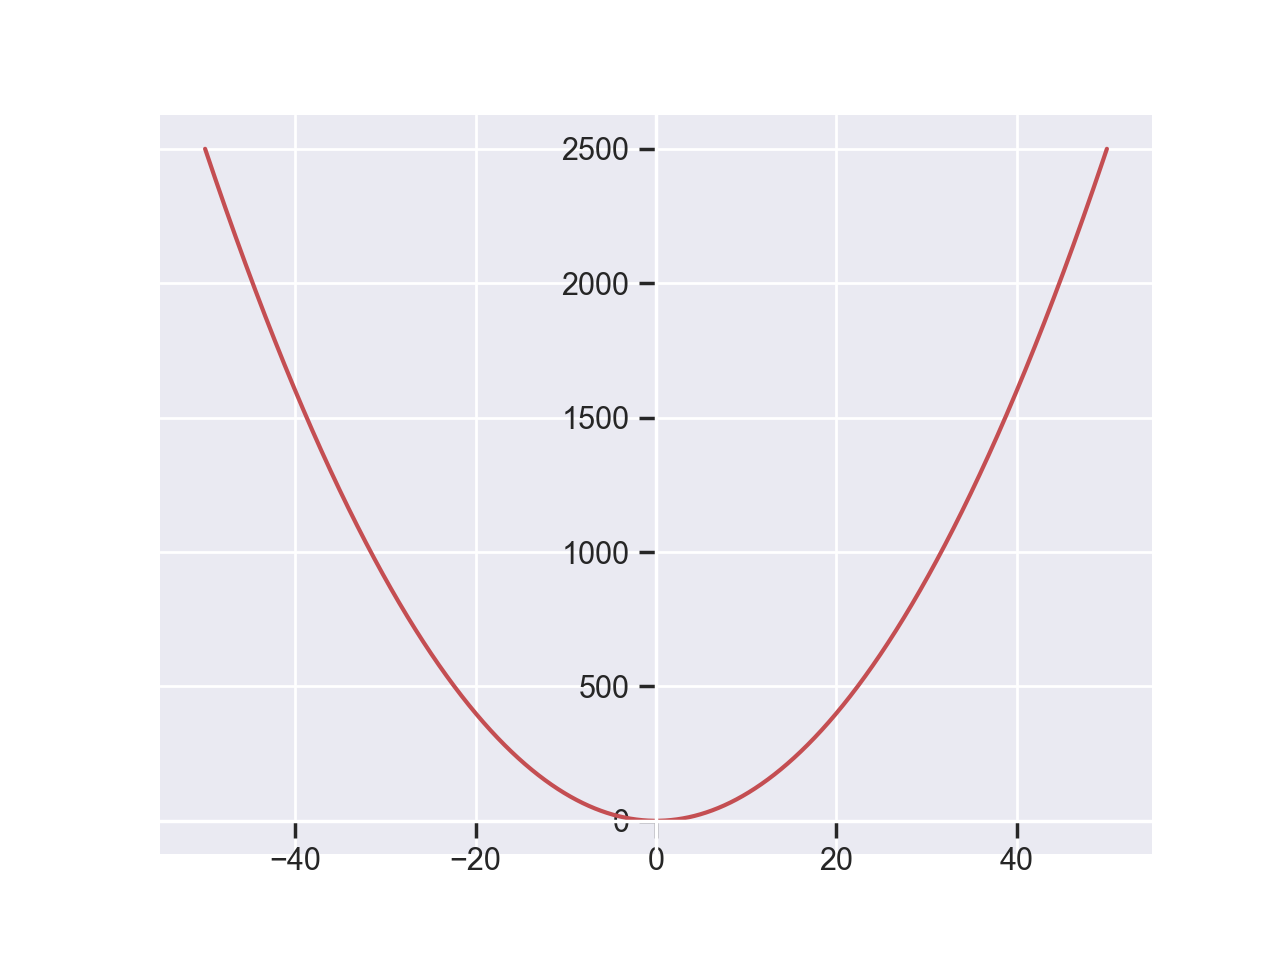
\includegraphics[width=6cm,height=6cm]{images/MSE}}}
	&\qquad\qquad
	\begin{aligned}
		MSE = \dfrac{1}{n} \sum_{i=1}^{n}(Y_i - \hat{Y}_i)^2
	\end{aligned}\\
	\vcenter{\hbox{\begin{minipage}{6cm}
				\captionof{figure}{نمودار تابع میانگین مربعات خطا بر اساس میزان خطا یا $\epsilon$}
	\end{minipage}}}
	& \notag
\end{align}
این تابع خطا نسبت به داده‌های پرت بسیار حساس بوده و ازین جهت جای بهبود دارد.

\subsubsection{میانگین قدرمطلق خطا}
این معیار خطا که به نوعی از نرم اول خطا استفاده می‌کند،‌ با جمع زدن از قدر مطلق خطا، معیاری از دقت عملکرد سیستم گزارش می‌دهد که رابطه‌ی آن به صورت زیر است:
\begin{align}
	\vcenter{\hbox{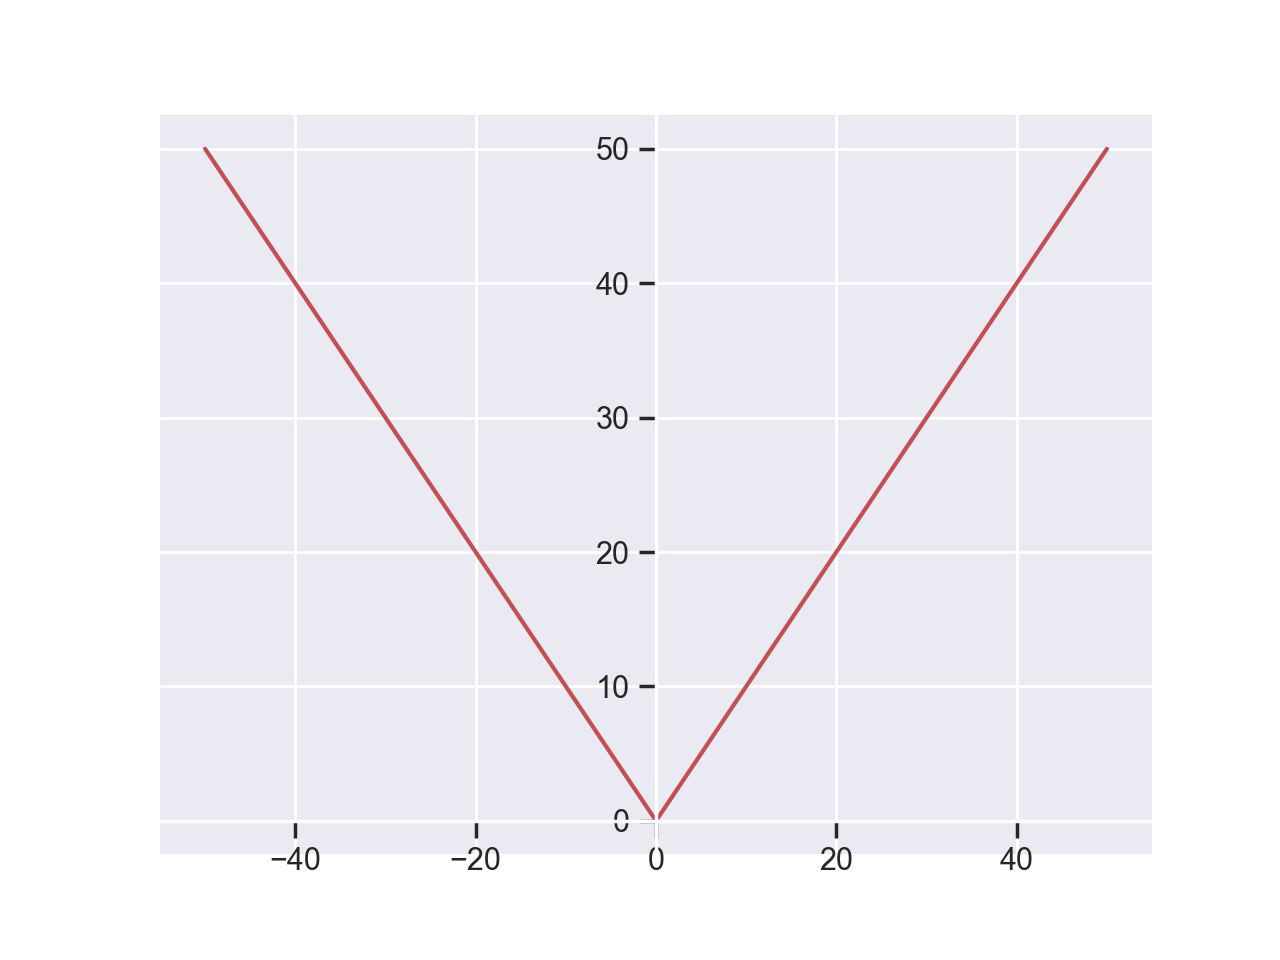
\includegraphics[width=6cm,height=6cm]{images/MAE}}}
	&\qquad\qquad
	\begin{aligned}
		MAE = \dfrac{1}{n} \sum_{i=1}^{n}|Y_i - \hat{Y}_i|
	\end{aligned}\\
	\vcenter{\hbox{\begin{minipage}{6cm}
				\captionof{figure}{نمودار میانگین قدرمطلق خطا بر اساس میزان خطا یا $\epsilon$}
	\end{minipage}}}
	& \notag
\end{align}
میانگین قدر مطلق خطا نسبت به تمامی نقاط موجود در مجموعه داده‌ رفتار یکسانی دارد. علت این امر آن است که شیب نمودار خطا به ازای تمامی مقادیر $\epsilon$ ثابت است و مانند میانگین مجموع مربعات خطا برای داده‌ها پرت افزایش نمیابد. ازین جهت می‌توان گفت که این تابع خطا نسبت به داده‌ها پرت حساسیت کمتری دارد.

\subsubsection{میانگین نسبی قدرمطلق خطا}
میانگین نسبی قدرمطلق خطا\LTRfootnote{Mean Absolute Percentage Error} مانند میانگین قدرمطلق خطا از نرم اول خطا برای محاسبه‌ی هزینه‌ی نهایی استفاده می‌کند، اما در مقابل این خطا را به مقدار ورودی اصلی تقسیم می‌کند که باعث می‌شود نوعی عادی سازی\LTRfootnote{Normalization} صورت بگیرد. رابطه‌ی این تابع خطا به صورت زیر است:
\begin{equation}
	MAPE = \dfrac{1}{n} \sum_{i=1}^{n}|\dfrac{Y_i - \hat{Y}_i}{\hat{Y}_i}|
\end{equation}
میانگین نسبی قدرمطلق خطا تابع خطای مناسبی برای سری‌های زمانی است. سری‌های زمانی اغلب با افزایش و کاهش‌های شدید در طول زمان مواجه هستند. در مقابل پیش‌بینی‌های انجام‌شده بر روی هر سری زمانی با خطاهایی همراه هست که با مقدار سری زمانی در آن نقطه نسبت مستقیمی دارند. به بیان دیگر با افزایش مقدار یک سری زمانی در طول زمان(به عنوان مثال افزایش نوسان بازار) پیش‌بینی آن با همان میزان خطای مطلق قبلی بسیار دشوارتر می‌شود و در نتیجه میزان خطای مدل نیز افزایش پیدا می‌کند. این مسئله باعث می‌شود تا مقادیر بزرگتر سری زمانی خطای بیشتری نسبی به مقادیر کوچک‌تر به مدل تحمیل کنند.\\
برای حل این مشکل تابع میانگین نسبی قدرمطلق خطا پیشنهاد شده است که با تقسیم مقدار مطلق خطا به مقدار سری زمانی در آن نقطه معیار بهتری از عملکرد سیستم نسبت به توابع دیگر به دست می‌دهد. از نگاهی دیگر این تابع خطا نسبت به افزایش و کاهش سری‌زمانی حساس نیست که باعث می‌شود خطای یکنواختی در طول سری زمانی ارائه کند. 
\newpage
\section{جمع‌بندی}
در این فصل با نحوه‌ی استخراج ویژگی‌ها مختلف از دفتر سفارشات آشنا شدیم و سپس به معرفی شبکه‌های عصبی بازگشتی و ساختار آن‌ها پرداختیم. در انتها نیز توابع خطای مورد استفاده در مطالعه‌ی سری‌های زمانی را معرفی کردیم. در فصل بعدی روش و جزییات پیاده سازی را تشریح می‌کنیم.


%\chapter{پیاده‌سازی و کتابخانه‌ها}

\section{مقدمه}
در این قسمت قصد داریم بخش پیاده‌سازی و کتابخانه‌های استفاده ‌شده را توضیح دهیم. پروژه با زبان برنامه‌نویسی پایتون پیاده‌سازی شده است. با توجه به معماری مدل‌های مبتنی بر شبکه‌های عصبی بازگشتی، برای پردازش با سرعت مناسب بهتر بود از پردازنده‌های گرافیکی\LTRfootnote{\lr{Graphics Processing Unit}} استفاده کنیم. به همین منظور، تمام کدهای پروژه بر روی سرویس کولب\LTRfootnote{\lr{Google Colaboratory}}، که به صورت رایگان امکان استفاده از پردازنده‌های گرافیکی به کاربران می‌دهد، اجرا شده است. در ادامه این بخش به تشریح قسمت‌های مختلف پیاده‌سازی و کتابخانه‌های استفاده ‌شده می‌پردازیم.

\section{واکشی و پیش‌پردازش دفتر ثبت سفارشات}
در این قسمت ابتدا نحوه‌ی واکشی اطلاعات دفتر ثبت سفارشات از صرافی آنلاین بایننس\LTRfootnote{Binance} به وسیله کتابخانه‌ی سی‌سی‌ایکس‌تی\LTRfootnote{ccxt} را تشریح می‌کنیم. سپس به نحوه‌ی ذخیره‌سازی سری‌های زمانی و ساخت مجموعه داده برچسب خورده برای یادگیری می‌پردازیم. در انتها نیز پیاده سازی مدل جی‌آريو و یادگیری مدل و تابع خطا را تشریح می‌کنیم.
\subsection{واکشی دفتر ثبت سفارشات}
هر رمز ارز در هر صرافی دارای دفتر سفارشات مخصوص به خود است. این دفاتر شامل سفارش‌های از جنس آن رمز ارز در آن صرافی هستند که بنا به سیاست هر صرافی می‌توان تاریخچه‌ی آن‌ها را درخواست کرد و مورد مطالعه قرار داد. در اینجا ما از داده‌های دفتر ثبت سفارشات صرافی بایننس که هم‌اکنون بزرگترین صرافی رمزارزها در دنیاست استفاده می‌کنیم. صرافی بایننس اجازه‌ی واکشی اطلاعات مربوط به دفتر سفارشات رمزارزهای گوناگونی که در آن مبادله می‌شوند را به کاربران خود می‌دهد که ما در این میان به مطالعه‌ی پنج رمزارز بزرگ‌تر می‌پردازیم.
\newpage
رمزارزهای مورد مطالعه:
\begin{itemize}
	\item بیتکوین\LTRfootnote{Bitcoin}
	\item اتریوم\LTRfootnote{Ethereum}
	\item بایننس کوین\LTRfootnote{Binance Coin}
	\item کاردانو\LTRfootnote{Cardano}
	\item دوج کوین\LTRfootnote{Doge Coin}
\end{itemize}
 اطلاعات مربوط به دفتر سفارشات این رمزارزها در صرافی بایننس و در بازه‌ی زمانی ابتدای ۲۰۲۰ تا ابتدای ۲۰۲۱ در این پروژه به کار گرفته شده است. برای واکشی اطلاعات مربوط به این رمزارز‌ها از کتابخانه‌ی سی‌سی‌ایکس‌تی\LTRfootnote{https://github.com/ccxt/ccxt} که یک کتابخانه‌ی مخصوص برای مطالعه و خرید و فروش رمز ارزهاست استفاده شده است.\\
 اطلاعات مربوط به هر رمزارز به صورت مجموعه‌ای از دفترهای سفارش در طول زمان و با فاصله‌ی زمانی یک دقیقه‌ای جمع‌آوری شده‌ است این دفترها که هرکدام موجودیتی سه‌بعدی هستند(شکل \ref{fig.orderbook_structure}) در طول زمان کنار یکدیگر قرار می‌گیرند و درنهایت یک آرایه‌ی چهاربعدی تشکیل می‌دهند. اما همانطور که پیش‌تر گفته شد این دفترها ابتدا به دفترهای سفارش تجمعی تبدیل می‌شوند و سپس قیمت میانی از آن‌ها استخراج می‌شود. به همین دلیل در ادامه، دیگر نیازی به دندانه‌های قیمت نخواهد بود چرا که فاصله‌ی آن‌ها توسط صرافی برابر مقدار ثابتی از مقدار میانی درنظر گرفته می‌شود و به همین دلیل نیازی به ذخیره‌سازی و وارد کردن این دندانه‌های با طول ثابت به مدل شبکه‌ی عصبی وجود نخواهد داشت. بر این اساس، با حذف دندانه‌های قیمت و ذخیره‌سازی حجم‌های متناظر مجموعه‌داده‌ی ورودی را تشکیل می‌دهیم.\\
 از طرف دیگر ویژگی‌هایی که در قسمت روش حل مسئله به آن‌ها اشاره کردیم را به مجموعه‌داده اضافه می‌کنیم که شامل قیمت میانی،
  شکاف قیمت، تغییر قیمت(بازده)، شکاف قیمت وزن‌دار و نوسان با دامنه‌های متفاوت است.\\
\begin{figure}[!t]
	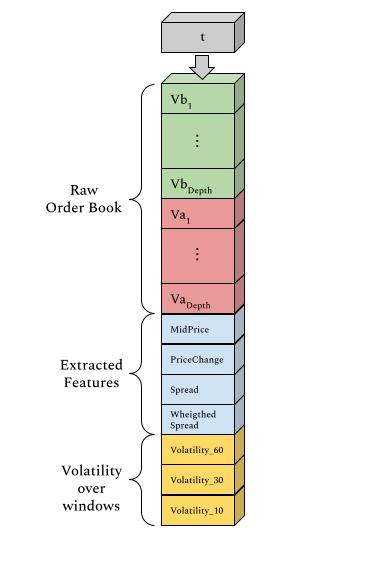
\includegraphics[width=0.5 \textwidth]{images/dataset_1}
	\centering
	\caption{اطلاعات ورودی به ازای هر لحظه‌ي $t$ در طول زمان	}
	\label{fig.dataset_1}
\end{figure}
بدین ترتیب در هر نقطه‌ از زمان مجموعه‌ای از اطلاعات جمع‌آوری و محاسبه می‌شود که می‌تواند برای یادگیری استفاده شود. در ادامه می‌توانیم با کنار هم قرار دادن دنباله‌ای از ستون‌هایی ازین جنس به یک یک ماتریس دست پیدا کنیم که هر ستون آن می‌تواند به یکی از واحد‌های مدل‌ جی‌آریو به عنوان ورودی داده شود.\\
هر دنباله‌ی ورودی که خود شامل تعدادی از ستون‌های شکل \ref{fig.dataset_1} است، می‌تواند توسط یک عدد که میزان نوسان در دقیقه‌ی آینده و یا پنج دقیقه‌ی آینده‌ی بعد از آن برچسب بخورد و برای آموزش به مدل داده شود. بنابراین نحوه‌ي برچسب‌زنی مجموعه‌ی نهایی به سه متغیر طول پنجره‌ی ورودی، حاشیه\LTRfootnote{Offset} و طول پنجره‌ی پیش‌بینی بستگی خواهد داشت(شکل \ref{fig.input_gru}).
\newpage
\begin{figure}[!t]
	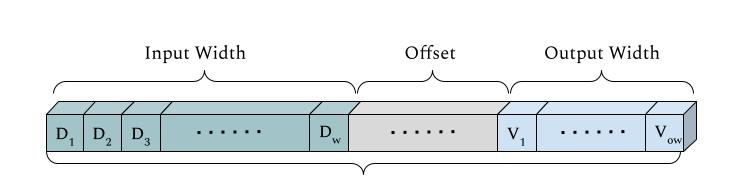
\includegraphics[width=1 \textwidth]{images/input_gru}
	\centering
	\caption{اطلاعات ورودی به ازای هر لحظه‌ي $t$ در طول زمان	}
	\label{fig.input_gru}
\end{figure}
به این صورت مجموعه‌داده نهایی به صورت مجموعه‌ای دنباله‌های ورودی با طول مشخص و برابر $W$ و خروجی متناظر با نوسان در بازه‌ای در آینده با طول $OW$ خواهد بود. طبیعی است که این مقادیر بسته به هدف استفاده از‌ مدل و توانایی پردازشی سیستم تعیین می‌شوند.
\section{مدل و یادگیری}
برای پیاده سازی مدل جی‌آریو از کتاب‌خانه‌ی تنسورفلو\LTRfootnote{Tensorflow} استفاده کرده‌ایم. این کتابخانه که مخصوص طراحی و آموزش شبکه‌های عصبی است، شامل پیاده‌سازی انواع مختلفی از شبکه‌های عصبیست که باعث شده در سال‌های گذشته به طور گسترده به کار گرفته شود.\\
\begin{figure}[!t]
	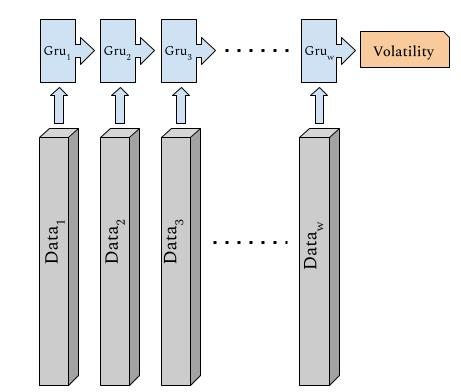
\includegraphics[width=0.6 \textwidth]{images/gru_function}
	\centering
	\caption{واردشدن اطلاعات ورودی به جی‌آریو برای تخمین نوسان}
	\label{fig.gru_function}
\end{figure}
\newpage
اطلاعات بدست آمده در مرحله‌ی قبل مانند شکل \ref{fig.gru_function} به عنوان ورودی به جی‌آریو داده می‌شوند و درنهایت به وسیله‌ی خطای محاسبه‌ شده آموزش داده می‌شود.
\section{جمع‌بندی}
در این فصل کتابخانه‌های استفاده شده را معرفی کردیم و به بیان جزییات ساخت مجموعه داده مورد استفاده پرداختیم. در ادامه به پیاده سازی شبکه‌ی عصبی جی‌آریو و نحوه‌ی انجام عمل یادگیری به وسیله‌ی داده‌های برچسب خورده پرداختیم.







%\chapter{ارزیابی}
%%%%%%%%%%%%%%%%%%%%%%%%%%%%%%%%%%%%%%%%%%%
\section{مقدمه}
در فصل‌های گذشته کارهای مرتبط انجام شده در این زمینه را معرفی کردیم. سپس به تشریح پیشنیاز‌ها و روش حل پیشنهادی برای حل مسئله پرداختیم. در ادامه وارد بخشی از جزییات پیاده سازی و ساخت مجموعه دادگان شدیم و نگاهی دقیق‌تر به این قسمت از پروژه داشتیم. در این فصل قصد داریم تا نتایج مدل‌نهایی را بر روی پنج رمزارز معرفی شده در فصل قبلی مشاهده و مقایسه کنیم و در نهایت به جمع‌بندی بپردازیم.

\section{مجموعه دادگان استفاده‌شده}
در این پروژه ما از سه مجموعه داده متین روتن تومیتوز، ای‌جی نیوز، و یلپ پولاریتی برای ارزیابی روش پیشنهادی‌مان استفاده کردیم. این مجموعه دادگان برای مساله دسته‌بندی تنظیم شده‌اند. در ادامه هر یک را به اختصار شرح می‌دهیم.

\begin{table}[!h]
	\caption{آمار و اطلاعات مربوط به دادگان روتن تومیتوز}
	\label{tomatoDataset}
	\begin{center}
		\begin{tabular}{|c|c|}
			\hline
			\textbf{آماره} & \textbf{مقدار} \\
			\hline
			\hline
			اندازه مجموعه آموزش
			&   ۸۵۳۰  \\
			\hline
			اندازی مجموعه اعتبارسنجی
			& ۱۰۶۶  \\
			\hline
			اندازه مجموعه آزمون
			& ۱۰۶۶ \\
			\hline
			میانگین طول خبر
			& ۲۰/۹۹  \\
			\hline
			
		\end{tabular}
	\end{center}
\end{table}

\begin{table}[!h]
	\caption{مثالی از عملکرد مدل بر روی یک حمله مخرب در دادگان روتن تومیتوز.}
	\label{tomatoex}
	\begin{center}
		\begin{tabular}{|c|c|}
			\hline
			
			\textbf{جمله اصلی} &
			
			\makecell{\lr{this is a fascinating film because there is no clear-cut hero} \\ \lr{and no all-out villain.}} \\ 
			\hline
			
			
			\textbf{مثال مخرب} &
			
			\makecell{\lr{this is a \textcolor{red}{fajscinating} film because there is no clear-cut hero} \\ \lr{and no all-out villain.}} \\ 
			\hline
			
			
			\textbf{عملکرد مدل} &
			
			\makecell{\lr{this is a \textcolor{blue}{fascinating} film because there is no clear-cut hero} \\ \lr{and no all-out villain.}} \\ 
			\hline
			
		\end{tabular}
	\end{center}
\end{table}

\subsection{مجموعه دادگان روتن تومیتوز}
دادگان این مجموعه از نظرات سایت تحلیل فیلم روتن تومیتوز\LTRfootnote{\lr{https://www.rottentomatoes.com/}} استخراج شده است. جدول \ref{tomatoDataset} مشخصات این مجموعه داده را نشان می‌دهد. این مجموعه دادگان برای مساله تحلیل احساسات بر روی دادگان متنی تنظیم شده است و دادگان آن دارای برچسب‌های "مثبت" و "منفی" هستند. در جدول \ref{tomatoex} یک نمونه از داده‌های این مجموعه دادگان و نحوه عملکرد مدل پیشنهادی ما بر روی آن را مشاهده می‌کنیم. 


\begin{table}[!h]
	\caption{آمار و اطلاعات مربوط به دادگان ای‌جی نیوز}
	\label{agDataset}
	\begin{center}
		\begin{tabular}{|c|c|}
			\hline
			\textbf{آماره} & \textbf{مقدار} \\
			\hline
			\hline
			اندازه مجموعه آموزش
			&   ۱۲۰۰۰۰  \\
			\hline
			اندازی مجموعه اعتبارسنجی
			& ۰  \\
			\hline
			اندازه مجموعه آزمون
			& ۷۶۰۰ \\
			\hline
			میانگین طول خبر
			& ۳۸/۴۱  \\
			\hline
			
		\end{tabular}
	\end{center}
\end{table}

\begin{table}[!h]
	\caption{مثالی از عملکرد مدل بر روی یک حمله مخرب در دادگان ای‌جی نیوز.}
	\label{agex}
	\begin{center}
		\begin{tabular}{|c|c|}
			\hline
			
			\textbf{جمله اصلی} &
			
			\makecell{\lr{Indian state rolls out wireless broadband Government in} \\ \lr{South Indian state of Kerala sets up wireless kiosks as part} \\ \lr{of initiative to bridge digital divide.}} \\ 
			\hline
			
		
			\textbf{مثال مخرب} &
			
			\makecell{\lr{Indian state rolls out wireless \textcolor{red}{broadbdand} Government in} \\ \lr{South \textcolor{red}{Indvian} state of Kerala sets up wireless kiosks as part} \\ \lr{of initiative to bridge digital \textcolor{red}{divside}.}} \\ 
			\hline
			
			
			\textbf{عملکرد مدل} &
			
			\makecell{\lr{Indian state rolls out wireless \textcolor{blue}{broadbdand} Government in} \\ \lr{South \textcolor{blue}{indian} state of Kerala sets up wireless kiosk as part} \\ \lr{of initiative to bridge digital \textcolor{blue}{divide}.}} \\ 
			\hline
			
		\end{tabular}
	\end{center}
\end{table}

\subsection{مجموعه دادگان ای‌جی نیوز}
مجموعه ای‌جی از بیش از ۱ میلیون متن خبری تشکیل شده است. این اخبار توسط موتور جست‌وجوی \lr{ComeToMyHead} و از بیش از ۲۰۰۰ منبع خبری جمع‌آوری شده‌اند. این موتور جست‌وجو مختص جست‌وجوی اخبار آکادمیک است و از سال ۲۰۰۴ مشغول جمع‌آوری اخبار است. از دادگان این مجموعه برای مسائل مختلف اعم از دسته‌بندی و خوشه‌بندی متن و مسائل مربوط به بازیابی اطلاعات استفاده شده است. مجموعه دادگان ا‌ی‌چی نیوز از این مجموعه توسط \cite{agnewsdata} به منظور استفاده در مساله دسته‌بندی متن معرفی شد. اخبار این مجموعه داده به چهار دسته "جهانی"، "ورزشی"، "تجارت"، و "فناوری و دانش" تقسیم می‌شوند. جدول \ref{agDataset} اطلاعات مربوط به این مجموعه داده را نشان می‌دهد. همچنین جدول \ref{agex} یک مثال از عملکرد مدل پیشنهادی ما بر روی یکی از خبرهای این مجموعه داده را نمایش می‌دهد.

\begin{table}[!h]
	\caption{آمار و اطلاعات مربوط به دادگان یلپ پولاریتی}
	\label{yelpDataset}
	\begin{center}
		\begin{tabular}{|c|c|}
			\hline
			\textbf{آماره} & \textbf{مقدار} \\
			\hline
			\hline
			اندازه مجموعه آموزش
			&   ۵۶۰۰۰۰  \\
			\hline
			اندازی مجموعه اعتبارسنجی
			& ۰  \\
			\hline
			اندازه مجموعه آزمون
			& ۳۸۰۰۰ \\
			\hline
			میانگین طول خبر
			& ۱35/63  \\
			\hline
			
		\end{tabular}
	\end{center}
\end{table}

\begin{table}[!h]
	\caption{مثالی از عملکرد مدل بر روی یک حمله مخرب در دادگان یلپ پولاریتی.}
	\label{yelpex}
	\begin{center}
		\begin{tabular}{|c|c|}
			\hline
			
			\textbf{جمله اصلی} &
			
			\makecell{\lr{A friendly place with great seafood. It is cash only. The clam} \\ \lr{chowder was meaty and creamy. The onion rings were crispy and} \\ \lr{so was the fish. A nice place to see local flair.}} \\ 
			\hline
			
			
			\textbf{مثال مخرب} &
			
			\makecell{\lr{A \textcolor{red}{fwriendly} place with \textcolor{red}{gresat} seafood. It is cash only. The clam} \\ \lr{chowder was meaty and \textcolor{red}{crreamy}. The onion rings were crispy and} \\ \lr{so was the fish. A nice place to see local flair.}} \\ 
			\hline
			
			
			\textbf{عملکرد مدل} &
			
			\makecell{\lr{A \textcolor{blue}{friendly} place with \textcolor{blue}{great} seafood. It is cash only. The clam} \\ \lr{chowder was meaty and \textcolor{blue}{creamy}. The onion rings were crisp and} \\ \lr{so was the fish. A nice place to see local flair.}} \\ 
			\hline
			
		\end{tabular}
	\end{center}
\end{table}

\subsection{مجموعه دادگان یلپ پولاریتی}
این مجموعه دادگان از تعداد بسیار زیادی تحلیل در سایت \lr{Yelp} و در یک چالش در سال ۲۰۱۵\LTRfootnote{Yelp Dataset Challenge 2015} تشکیل شده است. مجموعه دادگان یلپ پولاریتی توسط \cite{agnewsdata} از این دادگان استخراج شده است. این مجموعه داده برای مساله دسته‌بندی متن طراحی شده و دادگان آن دارای دو برچسب "مثبت" و "منفی" هستند. مشخصات این مجموعه داده در جدول \ref{yelpDataset} به نمایش درآمده و جدول \ref{yelpex} عملکرد مدل دفاعی ما برای یک مثال از این مجموعه داده را نشان می‌دهد.


\section{معیار ارزیابی}
برای ارزیابی مدل‌ها باید یک معیار ارزیابی مناسب که در حوزه یادگیری مخرب در متن استفاده شده است را معرفی کنیم.
\subsection{دقت}
معیار دقت\LTRfootnote{\lr{Accuracy}} معیاری‌ست که در ارزیابی مدل‌های دفاعی در برابر حملات مخرب بسیار به کار گرفته شده است. این معیار نسبت تعداد پیش‌بینی‌های صحیح به کل داده‌ها است. فرمول محاسبه این معیار در معادله \ref{eq:acc} آمده است.

\begin{equation} \label{eq:acc}
	Accuracy = \frac{TP + TN}{TP + TN + FP + FN}
\end{equation}
 
\section{نتایج}
در این بخش قسمت داریم نتایجی که در قسمت پیاده‌سازی به آن رسیده‌ایم را تشریح کنیم. به این منظور ابتدا مدل‌های پایه‌ای\LTRfootnote{\lr{Baseline}} که مورد استفاده قرار گرفته‌اند را معرفی می‌کنیم و سپس نتایج مدل پیشنهادی‌مان را بررسی می‌کنیم.
\subsection{مدل‌ پایه}
در مقالات مرتبط با سیستم‌های دفاعی در برابر حملات مخرب متنی به دلیل عدم عمومیت دادگان استفاده ‌شده عموما مدل‌های پایه‌ای مورد استفاده قرار گرفته‌اند که پیاده‌سازی آن‌ها توسط خود نویسندگان مقدور بوده باشد
\citep{jones2020robust, zhou2019learning, wang2019natural}.
 به دلیل گستردگی نوع حملات مخرب، دادگان واحدی که شامل دادگان مخرب واحد نیز باشد وجود ندارد به همین دلیل مدل‌های پایه‌ای که در مقالات این حوزه مورد استفاده قرار می‌گیرند باید قابلیت اجراشدن بر روی دادگان همان مقالات را داشته باشند. به همین دلیل ما در این پروژه روش شبکه‌های بازگشتی نیمه‌کاراکتری را که توانستیم بر روی دادگان مورد استفاده خود اجرا کنیم برای مدل‌ پایه در نظر گرفتیم.
\begin{itemize}
	\item{\textbf{مدل شبکه‌های بازگشتی نیمه‌کاراکتری}}:
	
	همانطور که در فصل ۲ بررسی کردیم استفاده از مدل‌های شبکه بازگشتی نیمه‌کاراکتری یکی از روش‌های استفاده‌‌شده در جهت دفاع در برابر حملات مخرب متنی بوده است. به همین دلیل تصمیم گرفتیم از این مدل به عنوان یک مدل پایه در ازیابی‌مان استفاده کنیم. برای این کار از مدل معرفی‌شده در مقاله \cite{sakaguchi2017robsut} برای پیش‌بینی و تصحصح مثال‌های مخرب متنی استفاده کردیم\LTRfootnote{\lr{https://github.com/keisks/robsut-wrod-reocginiton}}.
\end{itemize}

\subsection{نتایج مدل پیشنهادی}
در این بخش دقت‌های اندازه‌گیری شده روش پیشنهادی‌مان را بررسی می‌کنیم. همانطور که قبلا ذکر کردیم، برای بررسی عمکلرد مدل‌‌ها، سه دادگان یلپ پولاریتی، روتن تومیتوز و ای‌جی نیوز را انتخاب کردیم. برای مدل‌های اصلی دسته‌بند نیز از سه مدل برت، روبرتا و آلبرت که به صورت مدل‌های آماده در کتابخانه تکست‌اتک پیاده‌سازی شده‌اند استفاده کردیم. برای بررسی عملکرد دفاعی عملکرد مدل‌ها را بر روی مجموعه آزمون هر دادگان ارزیابی کردیم. برای این کار از هر مجموعه آزمون ۱۰۰۰ داده را انتخاب کردیم و بعد از مخرب‌سازی آن‌ها، عملکرد مدل‌های پایه و پیشنهادی را بر روی آن ۱۰۰۰ داده سنجیدیم. انتخاب ۱۰۰۰ داده به صورت تصادفی انجام شد و به این نکته توجه شد که از هر برچسب به میزان یکسان در ۱۰۰۰ داده نهایی وجود داشته باشد. جدول \ref{rotagtable} نتایج حاصل از عملکرد دفاعی مدل‌های پایه و مدل پیشنهادی‌مان بر روی دو دادگان روتن تومیتوز و ای‌جی‌ نیوز را نشان می‌دهد. جدول \ref{yelptable} نیز نتایج حاصل بر روی دادگان یلپ پولاریتی را نشان می‌دهد. همانطور که مشخص است عمکرد مدلی که بر اساس ویژگی پوشش واژه‌ها طراحی شده در تمام موارد از مدل پایه نیمه‌کاراکتری بهتر بوده است.


\begin{table}[h]
	\centering
	\caption{نتایج حاصل بر اساس معیار دقت بر روی دو دادگان ای‌جی نیوز و روتن تومیتوز.}
	\label{rotagtable}
	\begin{tabular}{ |c||c|c|c|c|c|c|c| }
		\hline
		\multicolumn{8}{|c|}{\textbf{جدول نتایج}} \\
		\hline
		\multirow{2}{*}{مدل} & \multirow{2}{*}{حمله} & \multicolumn{3}{|c|}{ای‌جی نیوز} & \multicolumn{3}{|c|}{روتن تومیتوز}\\\cline{3-8}
		
		&  & بی‌دفاع & ‌کاراکتری & پوشش واژه‌ & بی‌دفاع & ‌کاراکتری & پوشش واژه‌ \\
		\hline
		\multirow{3}{*}{\makecell{برت}}
		& اضافه & ۶۲/۰۰ & ۶۳/۶۰ & ۹۰/۵۰ & ۲۵/۷۰ & ‌۶۹/۳۲ & ۸۳/۰۲ \\
		& حذف  & ۶۱/۵۰ & ‌۶۴/۶۰ & ۸۶/۰۱ & ۲۱/۹۵ & ‌۶۸/۱۹ & ۷۱/۳۸ \\
		& جابه‌جایی  & ۶۳/۹۰ & ‌۶۶/۳۰ & ۸۹/۹۰ & ۴۷/۸۴ & ‌۷۱/۶۶ & ۷۹/۲۶\\\cline{3-8}
		& بدون حمله  & 
		\multicolumn{3}{|c|}{۹۳/۷۰} & \multicolumn{3}{|c|}{۸۵/۶۴} \\
		\hline
		\hline
		\multirow{3}{*}{\makecell{روبرتا}}
		& اضافه & ۶۵/۲۰ & ‌۶۴/۵۰ & ۸۸/۲۰ & ۳۰/۳۰ & ‌۷۴/۱۰ & ۸۴/۹۹ \\
		& حذف  & ۶۴/۳۰ & ‌۶۵/۸۰ & ۸۵/۳۰ & ۲۱/۴۸ & ‌۷۱/۰۱ & ۷۳/۷۳ \\
		& جابه‌جایی  & ۶۵/۹۰ & ‌۶۶/۹۰  & ۸۸/۵۰ & ۲۵/۴۲ & ‌۷۶/۰۷ & ۸۳/۳۰\\\cline{3-8}
		& بدون حمله  & 
		\multicolumn{3}{|c|}{۹۴/۳۰} & \multicolumn{3}{|c|}{۸۹/۰۲} \\
		\hline
		\hline
		\multirow{3}{*}{\makecell{آلبرت}}
		& اضافه & ۵۷/۲۰ & ‌۵۹/۲۰ & ۸۰/۰۰ & ۲۳/۱۷ & ‌۵۲/۱۵ & ۸۲/۲۷ \\
		& حذف  & ۵۵/۶۰ & ‌۵۹/۲۰ & ۷۶/۰۰ & ۱۷/۶۳ & ‌۵۱/۷۸ & ۷۳/۵۴ \\
		& جابه‌جایی  & ۵۹/۰۰ & ‌۶۱/۵۰  & ۸۰/۷۰ & ۲۰/۵۴ & ‌۵۳/۰۹ & ۸۰/۶۷\\\cline{3-8}
		& بدون حمله  & 
		\multicolumn{3}{|c|}{۸۵/۷۰} & \multicolumn{3}{|c|}{۸۵/۴۵} \\
		\hline
		
	\end{tabular}
\end{table}


\begin{table}[h]
	\centering
	\caption{نتایج حاصل بر اساس معیار دقت بر روی دادگان یلپ پولاریتی.}
	\label{yelptable}
	\begin{tabular}{ |c||c|c|c|c| }
		\hline
		\multicolumn{5}{|c|}{\textbf{جدول نتایج}} \\
		\hline
		\multirow{2}{*}{مدل} & \multirow{2}{*}{حمله} & \multicolumn{3}{|c|}{یلپ پولاریتی}\\\cline{3-5}
		
		&  & بی‌دفاع & ‌کاراکتری & پوشش واژه‌ \\
		\hline
		\multirow{3}{*}{\makecell{برت}}
		& اضافه & ۴۱/۰۶ & ‌۸۱/۴۰ & ۹۳/۷۰ \\
		& حذف  & ۳۵/۸۰ & ‌۷۹/۹۰ & ۸۷/۱۰ \\
		& جابه‌جایی  & ۴۲/۵۰ & ‌۸۳/۴۰ & ۹۲/۵۰\\\cline{3-5}
		& بدون حمله  & 
		\multicolumn{3}{|c|}{۹۷/۵۰}\\
		\hline
		\hline
		\multirow{3}{*}{\makecell{آلبرت}}
		& اضافه & ۳۳/۴۰ & ‌۷۹/۲۰ & ۹۵/۷۰ \\
		& حذف  & ۲۹/۸۰ & ‌۷۶/۴۰ & ۸۶/۹۰ \\
		& جابه‌جایی  & ۳۵/۱۰ & ‌۸۱/۷۰ & ۹۴/۰۰\\\cline{3-5}
		& بدون حمله  & 
		\multicolumn{3}{|c|}{۹۶/۹۰}\\
		\hline
		
	\end{tabular}
\end{table}


\section{جمع‌بندی}
در این فصل ابتدا به بررسی و توضیح ویژگی‌های دادگانی که در پروژه استفاده کرده‌ایم پرداختیم. در ادامه معیار ارزیابی‌ دقت که بر اساس آن می‌خواستیم نتایج کارمان را ارائه دهیم معرفی کردیم و در نهایت، نتایج مدل دفاعی‌مان را با مدل نیمه‌کاراکتری مقایسه کردیم. نتایج نشان دادند که عملکرد مدل ما بر روی هر سه دادگانی که مورد ارزیابی قرار گرفتند از مدل نیمه‌کاراکتری بهتر بوده است.

%\subsection{تحلیل نتایج}


%\chapter{جمع‌بندی، نتیجه‌گیری و پیشنهادات}
%%%%%%%%%%%%%%%%%%%%%%%%%%%%%%%%%%%%%%%%%%%
\section{جمع‌بندی و نتیجه‌گیری}
در این پروژه، در ابتدا مفهوم مثال مخرب در حوزه‌های بینایی ماشین و پردازش زبان طبیعی را مورد بررسی قرار دادیم. سپس روش‌های تولید مثال‌های مخرب و همچنین دفاع در برابر آن‌ها را توضیح دادیم. شرح دادیم که حملات مخرب در متن در سطوح مختلف کاراکتر، واژه، جمله و چندسطحی تعریف می‌شوند و راهکارهای دفاعی ارائه ‌شده در کارهای مرتبط در سال‌های اخیر بر دفاع در برابر یک شیوه حمله خاص تمرکز داشته‌اند. گفتیم که تمرکز ما در این پروژه بر دفاع برابر حملات مخرب متنی در سطح واژه به صورت غلط املایی است و چندی از مقالات مرتبط در زمینه دفاع در برابر حملات در سطح واژه را که از روش‌هایی مانند خوشه‌بندی و شبکه‌ عصبی بازگشتی استفاده کرده بودند معرفی کردیم. در قسمت روش پیشنهادی، ابتدا روش‌های مختلف بازنمایی متن را معرفی کردیم و به شرح مدل‌های مبتنی بر انتقال‌دهنده‌ها که اخیرا در مسائل مختلف حوزه پردازش زبان استفاده شده‌اند پرداختیم. توضیح دادیم که چگونه می‌توان با استفاده از ویژگی پوشش واژ‌ه‌ها در مدل برت یک معیار برای امتیازدهی به معناداری کلمات در یک جمله در نظر گرفت و بر اساس این معیار تشخیص داد کدام واژه در یک جمله احتمالا یک واژه مخرب است. سپس برای تصحیح واژگانی که مخرب شناخته‌ شده‌اند، از لغت‌نامه گلاو استفاده کردیم تا با بررسی تمام همسایگان کاراکتری واژه مخرب متوجه شویم کدام یک از این همسایگان کلمه‌ای بامعنی است و در نهایت واژه‌ای که بیشترین امتیاز معناداری را داشته باشد به عنوان جایگزین کلمه مخرب معرفی می‌کردیم. در قسمت پیاده‌سازی نیز کتابخانه‌های تکست‌اتک و هاگینگ‌فیس و چگونگی استفاده ما از آن‌ها برای تولید مثال‌های مخرب و مدل‌های از پیش‌ آموزش‌دیده را توضیح دادیم. در نهایت نتایج مدل پیشنهادی‌مان را بر روی سه دادگان یلپ پولاریتی، روتن تومیتوز و ای‌جی نیوز ارائه کردیم و نشان دادیم در تمام نتایج عملکرد مدل‌مان از روش نیمه‌کاراکتری بهتر بوده است.

\section{پیشنهادات}
همانطور که در بخش مقدماتی پروژه اشاره شد، روش‌های متنوعی برای تولید حملات مخرب در متن تا کنون ارائه شده است. روشی که با استفاده از پوشش واژه‌ها در برت ارائه دادیم قابلیت تشخیص حملات در سطح کلمه چه به صورت غلط املایی و چه به صورت مترادف را دارد. بنابراین یکی از پیشنهادات ما در این حوزه طراحی مدلی برای تصحیح کلمات مخرب تشخیص‌ داده‌شده‌ای است که به صورت مترادف کلمات اصلی به کار گرفته شده‌اند. همچنین با توجه به بار محاسباتی بالای محاسبه امتیاز جملات با استفاده از ویژگی پوشش واژه‌ها، ارائه راهکاری برای کمینه‌کردن این امر در هنگام پردازش داده‌ها می‌تواند کمک شایانی به تسریع و بهبود کیفیت روند پروژه نماید.

%--------------------------------------------------------------------------appendix( مراجع و پیوست ها)
\chapterfont{\vspace*{-2em}\centering\LARGE}%

\appendix
\bibliographystyle{plain-fa}
\bibliography{references}
\chapter*{‌پیوست}
\markboth{پیوست}{}
\addcontentsline{toc}{chapter}{پیوست}

\begin{latin}
\section*{\lr{English Summary}}
\lr{Nowadays, machine learning models are widely used in varied applications and issues. One of the important challenges for these models, especially deep ones, is adversarial learning and adversarial examples which are generated especially for machine learning models. Natural Language Processing is also an area in which adversarial learning and adversarial examples should be considered as a major concern. In this project, our purpose is to devise a defense system against text adversarial examples generated to fool NLP models. Masked language modeling, one of the phases in pretraining of deep BERT, is used to design an approach to identify adversarial examples in text. We also use pre-trained word embeddings (GLOVE) to find the correct form of those words identified as adversarial. To evaluate our method, the performance of our defense system is measured on three transformer-based models and three english text classification datasets. The results show that our method outperforms semi-character neural networks, another novel defensive method against text adversarial examples, in all experiments.}
\end{latin}
%--------------------------------------------------------------------------dictionary(واژه نامه ها)
%اگر مایل به داشتن صفحه واژه‌نامه نیستید، خط زیر را غیر فعال کنید.
%\parindent=0pt
%%
\chapter*{واژه‌نامه‌ی فارسی به انگلیسی}
\pagestyle{style9}

\addcontentsline{toc}{chapter}{واژه‌نامه‌ی فارسی به انگلیسی}
%%%%%%
\begin{multicols*}{2}

{\bf آ}
\vspace*{3mm}


\farsiTOenglish{اسکالر}{Scalar}


\vspace*{3mm}
{\bf ب}
\vspace*{3mm}

\farsiTOenglish{بالابر}{Lift}


\vspace*{3mm}
{\bf پ}
%%\vspace*{3mm}

\farsiTOenglish{پایا}{Invariant}



\vspace*{3mm}
{\bf ت}
%%\vspace*{3mm}

\farsiTOenglish{ تناظر }{Correspondence}


\vspace*{3mm}
{\bf ث}
%%\vspace*{3mm}

\farsiTOenglish{ثابت‌ساز}{Stabilizer}

\vspace*{3mm}
{\bf ج}
%%\vspace*{3mm}

\farsiTOenglish{جایگشت}{Permutation}



\vspace*{3mm}
{\bf چ}
%%\vspace*{3mm}


\farsiTOenglish{چند جمله‌ای }{Polynomial}

\vspace*{3mm}
{\bf ح}
%%\vspace*{3mm}

\farsiTOenglish{حاصل‌ضرب دکارتی}{Cartesian product}


\vspace*{3mm}
{\bf خ}
%%\vspace*{3mm}

\farsiTOenglish{خودریختی}{Automorphism}

\vspace*{3mm}
{\bf د}
%%\vspace*{3mm}

\farsiTOenglish{درجه}{Degree}


\vspace*{3mm}
{\bf ر}
%%\vspace*{3mm}


\farsiTOenglish{ریزپردازنده}{microprocessor}


\vspace*{3mm}
{\bf ز}
%%\vspace*{3mm}


\farsiTOenglish{زیرمدول}{Submodule}


\vspace*{3mm}
{\bf س}
%%\vspace*{3mm}

\farsiTOenglish{سرشت}{Character}


\vspace*{3mm}
{\bf ص}
%%\vspace*{3mm}

\farsiTOenglish{صادقانه}{Faithful}

\vspace*{3mm}
{\bf ض}
%%\vspace*{3mm}

\farsiTOenglish{ضرب داخلی}{Inner product}

\vspace*{3mm}
{\bf ط}
%%\vspace*{3mm}


\farsiTOenglish{طوقه}{Loop}


\vspace*{3mm}
{\bf ظ}
%%\vspace*{3mm}


\farsiTOenglish{ظرفیت}{Valency}
 
\vspace*{3mm}
{\bf ع}
%%\vspace*{3mm}


\farsiTOenglish{عدم مجاورت}{Nonadjacency}



\vspace*{3mm}
{\bf ف}
%%\vspace*{3mm}

\farsiTOenglish{فضای برداری}{Vector space}



\vspace*{3mm}
{\bf ک}
%%\vspace*{3mm}

\farsiTOenglish{کاملاً تحویل‌پذیر}{Complete reducibility}


\vspace*{3mm}
{\bf گ}
%%\vspace*{3mm}


\farsiTOenglish{گراف}{Graph}



\vspace*{3mm}
{\bf م}
%%\vspace*{3mm}

\farsiTOenglish{ماتریس جایگشتی}{Permutation matrix }


\vspace*{3mm}
{\bf ن}
%%\vspace*{3mm}

\farsiTOenglish{ناهمبند}{Disconnected}


\vspace*{3mm}
{\bf و}
%%\vspace*{3mm}

\farsiTOenglish{وارون‌پذیر}{Invertible}


\vspace*{3mm}
{\bf ه}
%%\vspace*{3mm}

\farsiTOenglish{همبند}{Connected}



\vspace*{3mm}
{\bf ی}
%%\vspace*{3mm}

\farsiTOenglish{یال}{Edge}




\end{multicols*}%
%%%%%%%
\chapter*{ واژه‌نامه‌ی انگلیسی به فارسی}
\pagestyle{style9}
\lhead{\thepage}\rhead{واژه‌نامه‌ی انگلیسی به فارسی}
\addcontentsline{toc}{chapter}{واژه‌نامه‌ی انگلیسی به فارسی}

\LTRmulticolcolumns
\begin{multicols}{2}
{\hfill\bf  \lr{A}}
%%\vspace*{1.5mm}

\englishTOfarsi{Automorphism}{خودریختی}

\vspace*{3mm}
{\hfill\bf   \lr{B}}
%%\vspace*{1.5mm}

\englishTOfarsi{Bijection}{دوسویی}

\vspace*{3mm}
{\hfill\bf   \lr{C}}
%%\vspace*{1.5mm}

\englishTOfarsi{Cycle group}{گروه دوری}

\vspace*{3mm}
{\hfill\bf   \lr{D}}
%%\vspace*{1.5mm}

\englishTOfarsi{Degree}{درجه}

\vspace*{3mm}
{\hfill\bf   \lr{E}}
%%\vspace*{1.5mm}

\englishTOfarsi{Edge}{یال}

\vspace*{3mm}
{\hfill\bf   \lr{F}}
%%\vspace*{1.5mm}

\englishTOfarsi{Function}{تابع}

\vspace*{3mm}
{\hfill\bf   \lr{G}}
%%\vspace*{1.5mm}

\englishTOfarsi{Group}{گروه}

\vspace*{3mm}
{\hfill\bf   \lr{H}}
%%\vspace*{1.5mm}

\englishTOfarsi{Homomorphism}{همریختی}

\vspace*{3mm}
{\hfill\bf   \lr{I}}
%%\vspace*{1.5mm}

\englishTOfarsi{Invariant}{پایا}

\vspace*{3mm}
{\hfill\bf   \lr{L}}
%%\vspace*{1.5mm}

\englishTOfarsi{Lift}{بالابر}

\vspace*{3mm}
{\hfill\bf   \lr{M}}
%%\vspace*{1.5mm}

\englishTOfarsi{Module}{مدول}

\vspace*{3mm}
{\hfill\bf   \lr{N}}
%%\vspace*{1.5mm}

\englishTOfarsi{Natural map}{نگاشت طبیعی}

\vspace*{3mm}
{\hfill\bf   \lr{O}}
%%\vspace*{1.5mm}

\englishTOfarsi{One to One}{یک به یک}

\vspace*{3mm}
{\hfill\bf   \lr{P}}
%%\vspace*{1.5mm}

\englishTOfarsi{Permutation group}{گروه جایگشتی}

\vspace*{3mm}
{\hfill\bf   \lr{Q}}
%%\vspace*{1.5mm}

\englishTOfarsi{Quotient graph}{گراف خارج‌قسمتی}

 \vspace*{3mm}
{\hfill\bf   \lr{R}}
%%\vspace*{1.5mm}

\englishTOfarsi{Reducible}{تحویل پذیر}

\vspace*{3mm}
{\hfill\bf   \lr{S}}
%%\vspace*{1.5mm}

\englishTOfarsi{Sequence}{دنباله}

 \vspace*{3mm}
{\hfill\bf   \lr{T}}
%%\vspace*{1.5mm}

\englishTOfarsi{Trivial character}{سرشت بدیهی}

\vspace*{3mm}
{\hfill\bf   \lr{U}}
%%\vspace*{1.5mm}

\englishTOfarsi{Unique}{منحصربفرد}

\vspace*{3mm}
{\hfill\bf   \lr{V}}
%%\vspace*{1.5mm}

\englishTOfarsi{Vector space}{فضای برداری}
\end{multicols}
%--------------------------------------------------------------------------index(نمایه)
%اگر مایل به داشتن صفحه نمایه نیستید، خط زیر را غیر فعال کنید.
%\pagestyle{style7}
%\printindex
%\pagestyle{style7}
%%کلمات کلیدی انگلیسی
\latinkeywords{Write a 3 to 5 KeyWords is essential. Example: AUT, M.Sc., Ph. D,..}
%چکیده انگلیسی

\en-abstract{
This page is accurate translation from Persian abstract into English.
}
%%%%%%%%%%%%%%%%%%%%% کدهای زیر را تغییر ندهید.

\newpage
\thispagestyle{empty}
\begin{latin}
\section*{\LARGE\centering Abstract}

\een-abstract

\vspace*{.5cm}
{\large\textbf{Key Words:}}\par
\vspace*{.5cm}
\elatinkeywords
\end{latin}
%% در این فایل، عنوان پایان‌نامه، مشخصات خود و چکیده پایان‌نامه را به انگلیسی، وارد کنید.
%%%%%%%%%%%%%%%%%%%%%%%%%%%%%%%%%%%%
\baselineskip=.6cm
\begin{latin}

\latinfaculty{Department of ...}


\latintitle{Title of Thesis}


\firstlatinsupervisor{Dr. }

%\secondlatinsupervisor{Second Supervisor}

\firstlatinadvisor{Dr. }

%\secondlatinadvisor{Second Advisor}

\latinname{Name}

\latinsurname{Surname}

\latinthesisdate{Month \& Year}

\latinvtitle
\end{latin}

\end{document}